\documentclass[8pt,compress,aspectratio=169]{beamer}
\usepackage{multicol}
\usepackage{graphics}
%\usepackage{cascadia-code}
\usepackage{listings}
\usepackage{soul}
\usepackage[default]{sourcesanspro}
\usepackage[T1]{fontenc}
\usepackage[font=tiny]{caption}
%\renewcommand*\familydefault{\ttdefault} %% Only if the base font of the document is to be typewriter style
\newcommand\LightBold[1]{\textcolor{VSBlueLight}{\textbf{#1}}}
\newcommand\DarkBold[1]{\textcolor{VSBlueDark}{\textbf{#1}}}
\newcommand\DarkBoldP[1]{\textcolor{VSPurpleDark}{\textbf{#1}}}
\usepackage[T1]{fontenc}

\usetheme{Dark}


% Title Slide
\title{Claims Investigation Committee Multi-Testing Input Device}
\subtitle{ECE-4820: Electrical and Computer Engineering Design II}
\author[Garza, Baker, Sah]{Dylan-Matthew Garza \and Daniel Baker \and Rohullah Sah \and}

\institute[VFU] % (optional)
{
      Department of Electrical and Computer Engineering\\
      Western Michigan University
      \and
      ZF Group\\
      Auburn Hills, MI
}
\date{Fall 2024}
\titlegraphic{
\includegraphics[height=2cm]{assets/WMU_Logo.png}\hspace{1cm}
\includegraphics[height=2cm]{assets/zf.png}}



\begin{document}
%==============================================================================
% Introduction slide
%==============================================================================
\begin{frame}[plain]
  \titlepage
  \small
  \begin{multicols}{2}
      Faculty Advisor:\\
      Dr. Janos Grantner\hfill\\
    \hfill{}\makebox[0pt][r]{Sponsor Manager}:\\
    \hfill Patrick McNally
  \end{multicols}
\end{frame}

\AtBeginSection[]
{
  \begin{frame}
    \frametitle{Table of Contents}
    \tableofcontents[currentsection]
  \end{frame}
}
\section{Introduction}

%==============================================================================
% INTRODUCTION SECTION
%==============================================================================
\subsection{ZF}
\begin{frame}
  \frametitle{ZF}
  \begin{minipage}{0.45\textwidth}
    \begin{block}{Who is ZF?}
      \begin{itemize}
          \small {
            \item Global technology company and Tier 1 automotive supplier
            \item Provides advanced safety systems and vehicle control solutions
            \item Partners with major OEMs: Daimler, Chrysler, Tesla, Waymo(Google), etc.
            \item A leading innovator in commercial vehicle technology
          }
      \end{itemize}
    \end{block}
    \begin{block}{North American Headquarters}
      \begin{itemize}
          \small {
            \item Project based at ZF Group's North American headquarters in Auburn Hills, MI
            \item Specializes in commercial vehicle solutions
            \item This facility is also home to the Claims Investigation Center
            }
      \end{itemize}
    \end{block}
  \end{minipage}
  \hfill
  \begin{minipage}{0.45\textwidth}
    \begin{figure}
      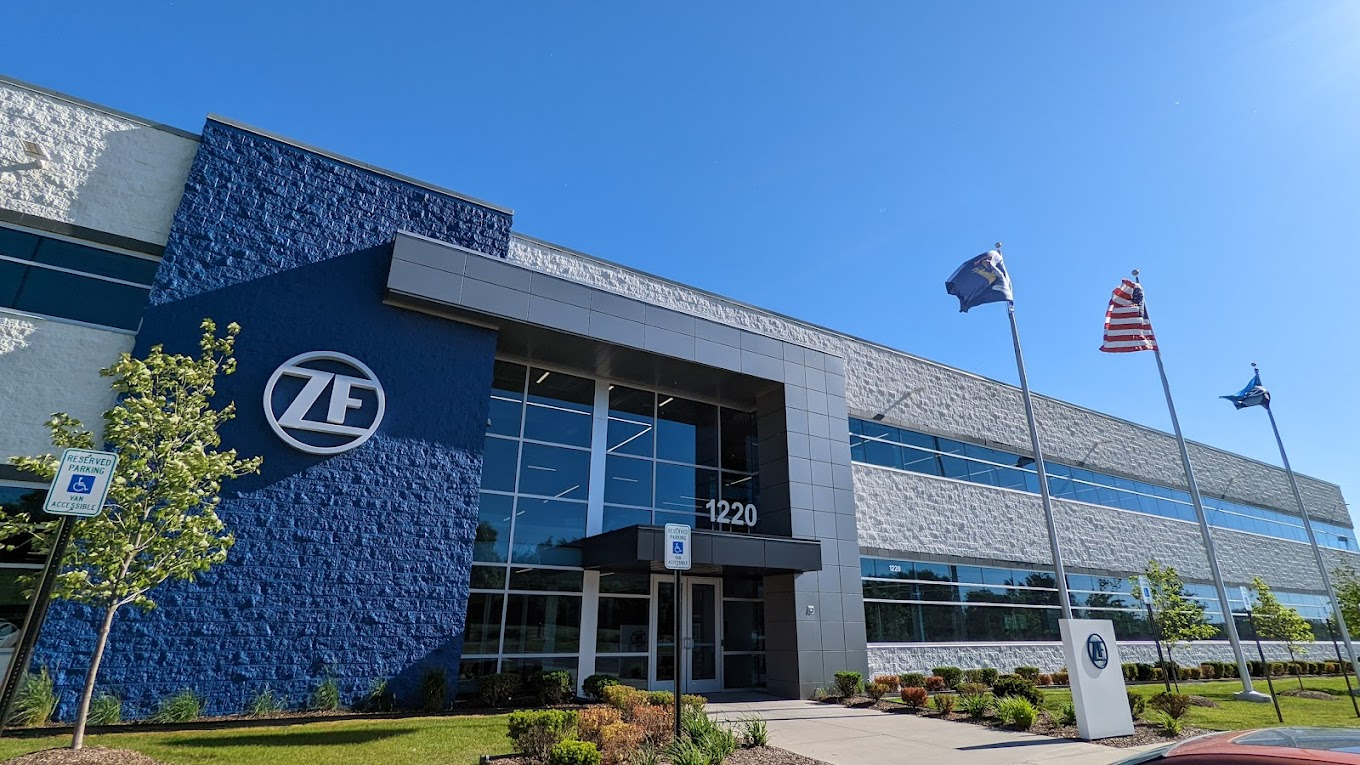
\includegraphics[width=\textwidth]{assets/misc/zf-office.jpg}
      \caption{Source: \href{google.com}{google.com}\hspace{\textwidth}
      \textit{ZF Group Office in Auburn Hills, MI}}
    \end{figure}
  \end{minipage}
\end{frame}

\subsection{Claims Investigation Committee}
\begin{frame}
  \frametitle{Claims Investigation Committee}
  \begin{block}{What is the Claims Investigation Center?}
      \begin{itemize}
          \small {
            \item Specialized team focused on testing and initial investigation of field failure parts for commercial vehicles 
            \item Identifies new field failures and determine areas for product improvement
            \item Works closely with Technical Call Centers, Field Quality, and Warranty teams
            \item Ensures readiness to test and analyze new product field returns at launch  
          }
      \end{itemize}
  \end{block}


  \begin{block}{CIC's Role in Our Project}
    \begin{itemize}
        \small {
          \item Requires enhanced testing capabilites for new products
          \item Our project aims to develop a device to streamline testing and data collection
          \item Helps the CIC efficiently validate warranty claims and analyze field returns
          \item Supports the CIC's mission to improve product quality and customer satisfaction
          }
    \end{itemize}
  \end{block}
  \end{frame}

\subsection{Project Motivation}
\begin{frame}
    \frametitle{Motivation for the Project}
    \begin{minipage}{0.475\textwidth}
    \begin{block}{Challenges with Current Testing Methods}
        \begin{itemize}
            \small
            \item Testing on current brake system platform (mBSP) was built and industrialized specifically for that platform
            \item Long lead time and significant cost to release and document
            \item New platform components are not compatible with the current tester
            \item Current tester is not capable of testing in prototype phase
        \end{itemize}
    \end{block}
    \begin{block}{Need for Improvement}
      \small
        \begin{itemize}
          \item The Brake Signal Transmitter's (BST) implementation in Daimler's new platform intensifies urgency
            \item High production volumes require efficient testing methods 
            \item Expanding product line increases testing complexity
        \end{itemize}
    \end{block}
    \end{minipage}
    \hfill
    \begin{minipage}{0.475\textwidth}
        \begin{figure}
          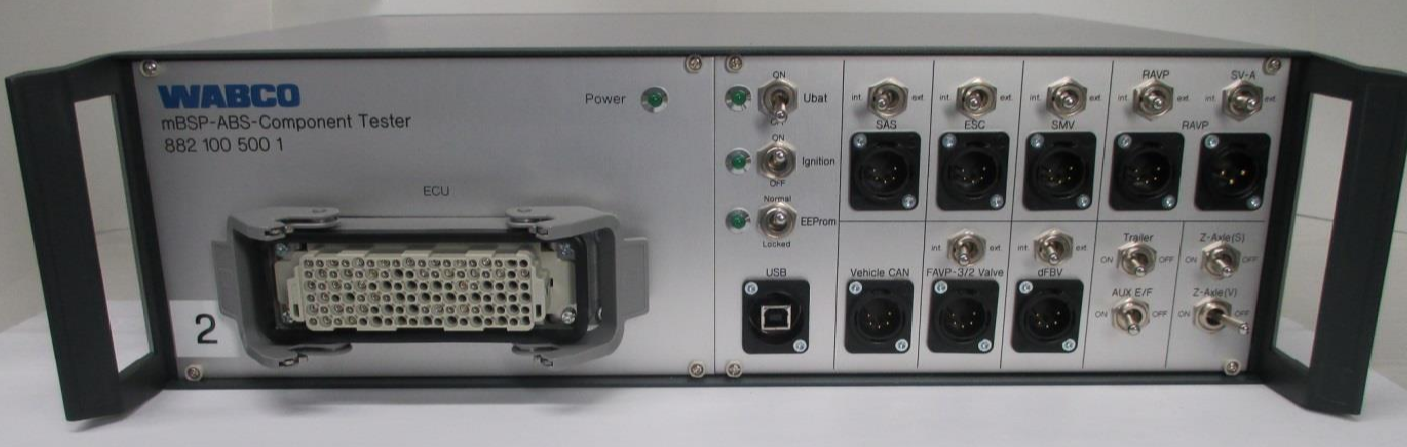
\includegraphics[width=\textwidth]{assets/misc/abs-tester.png}
          \caption{\it Current brake component system tester}
        \end{figure}
    \end{minipage}
\end{frame}


\subsection{Our Solution}
\begin{frame}
    \frametitle{Multi-Testing Input Device}
    \begin{block}{Addressed Challenges}
        \begin{itemize}
            \item Provides a unified testing platform for multiple devices
            \item Flexible and agile to adapt to new product lines
            \item Allows for prototype testing and validation
            \item Automates data collection and analysis to reduce time and errors
            \item Increases testing speed and accuracy
            \item Simplifies validation process for warranty claims
            \item Enhances capability to analyze field returns efficiently
            \item Cost-effective solution
        \end{itemize}
    \end{block}
\end{frame}

\subsection{Key Devices Under Test}
\begin{frame}
    \frametitle{Devices Our Solution Supports}
    \begin{block}{Key Devices Under Test (DUTs)}
    \begin{enumerate}
        \item {\DarkBold{Brake Signal Transmitter (BST)}}
        \begin{itemize}
            \item Primary focus - critical new component for 2025 production
            \item Acts as the brain that reads how hard a driver presses the brake.
        \end{itemize}
        \item {\DarkBold{Continuous Wear Sensor (CWS)}}
        \begin{itemize}
            \item Works like a monitor for your brake pads and discs
            \item Warns when brakes are wearing down using voltage
        \end{itemize}
        \item {\DarkBold{Pressure Sensor}}
        \begin{itemize}
            \item Continuously measures relative pressure in vehicle control systems
        \end{itemize}
        \item {\DarkBold{Electronic Stability Control Module (ESCM)}}
            \begin{itemize}
                \item Acts as a safety system that helps prevent skidding and rollovers
                \item Monitors the vehicle's movement and intervenes to keep it stable
            \end{itemize}
    \end{enumerate}
  \end{block}
\end{frame}

%==============================================================================
% DESIGN AND IMPLEMENTATION SECTION: Project Solution and Overview
%==============================================================================
\section{Design and Implementation}
\subsection{Project Solution and Overview}

\begin{frame}
  \frametitle{Project Solution}
  \centering
  \includegraphics[width=0.5\textwidth]{assets/diagrams/hardware.png}
  \begin{block}{What this project aims to accomplish:}
    \begin{enumerate}
      \item {\DarkBold{Device Interfacing}}
        \begin{enumerate}
          \item Properly read Device Signals using the ARM Cortex-M4 on the onboard microcontroller on the 
            \LightBold{STM32MP157F-DK2}:
            \begin{itemize}
              \item PWM Duty Cycle
              \item Frequency
              \item Voltages through an analog-to-digital converter (ADC)
              \item CAN frames
            \end{itemize}
        \end{enumerate}
      \item \DarkBold{Physical Components and Hardware}
        \begin{enumerate}
          \item Printed Circuit Board (PCB) for interfacing with DUT
          \item PCB for scaling and managing power for the DUT and to the microcontroller
          \item Enclosure for PCBs and \LightBold{STM32MP157F-DK2} board
        \end{enumerate}
    \end{enumerate}
  \end{block}
\end{frame}

\begin{frame}
  \frametitle{Project Solution (cont.)}
  \begin{block}{What this project aims to accomplish:}
    \begin{enumerate}
        \setcounter{enumi}{2}
        \large
      \item \DarkBold{Software}
        \begin{enumerate}
            \large
          \item Custom embedded \textbf{Linux} distribution that will run on the onboard ARM Cortex-A7
            microprocessor on the \LightBold{STM32MP157F-DK2}
          \item Simple user interface on web-based application
          \item Custom Webserver to process information from web application to microcontroller
          \item Communicate collected information from ARM Cortex-M4 to ARM Cortex-A7
          \item Ability to download measured data, formatted as a CSV, through the web application 
        \end{enumerate}
    \end{enumerate}
  \end{block}
\end{frame}

\begin{frame}
  \frametitle{Comprehensive System Block Diagram}
  \centering
  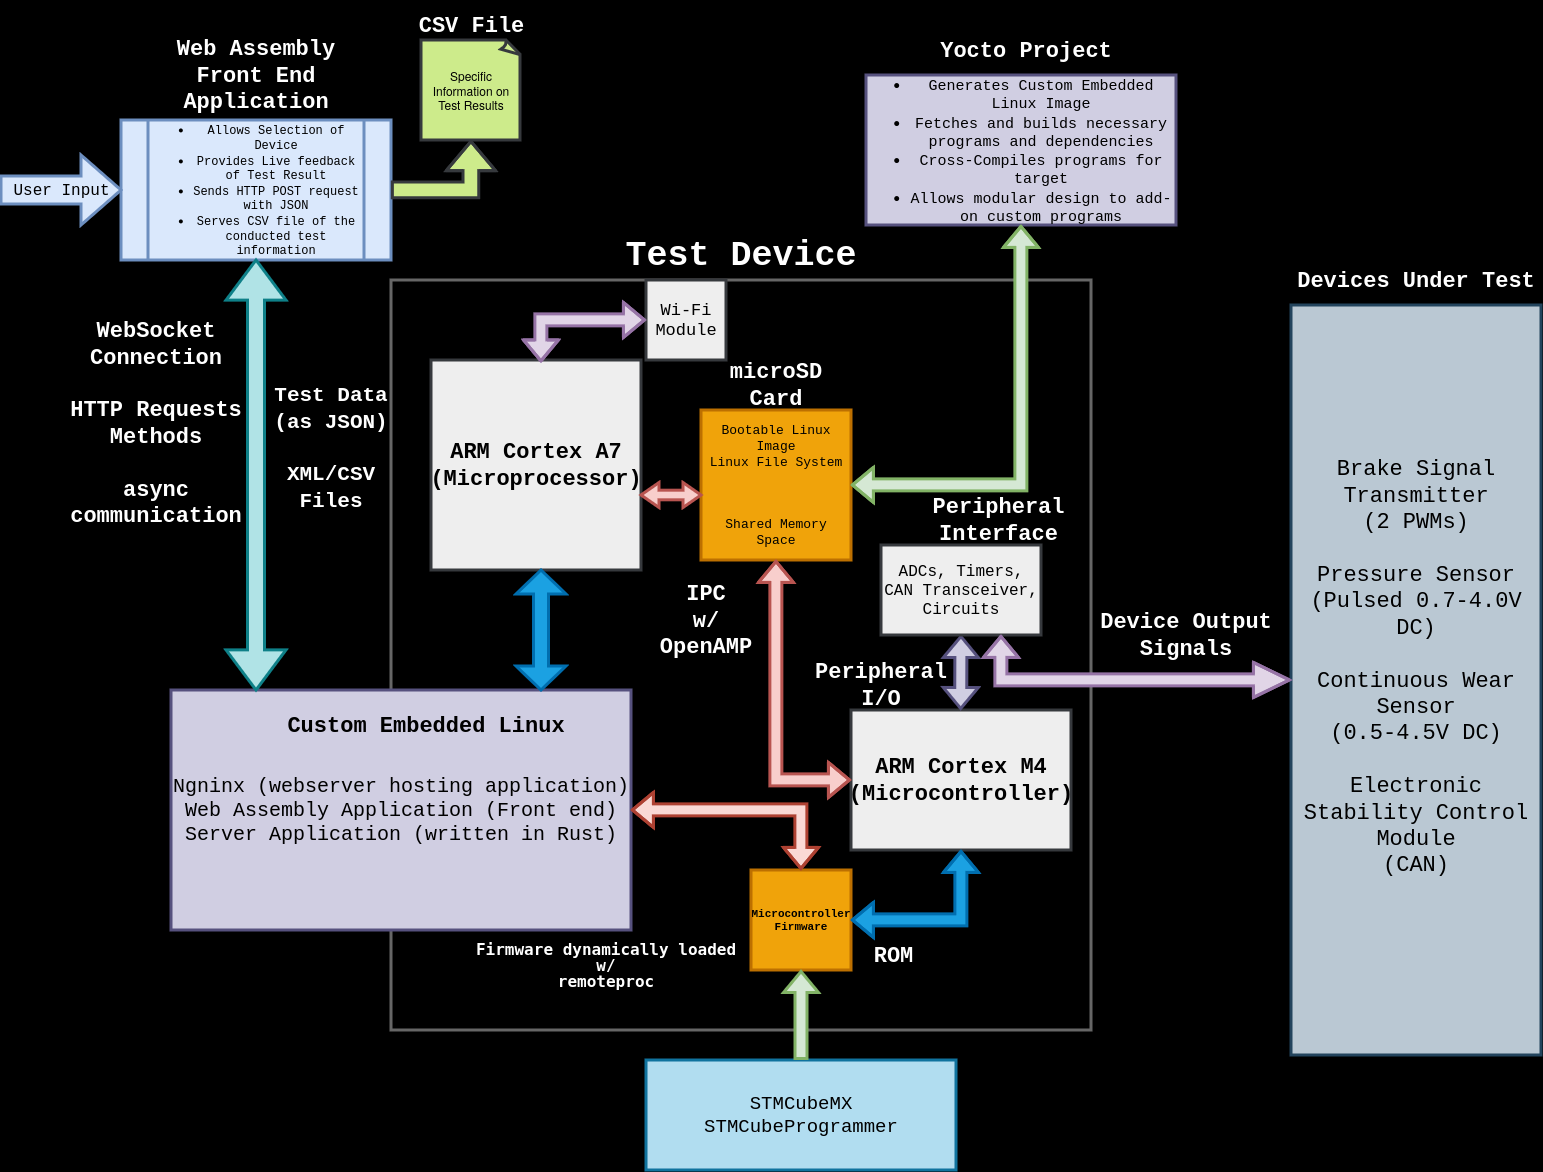
\includegraphics[height=0.85\paperheight]{assets/diagrams/block_diagram.drawio.png}
\end{frame}
 
%==============================================================================
% DESIGN AND IMPLEMENTATION SECTION: Gantt Chart
%==============================================================================
\begin{frame}
  \frametitle{Gantt Chart}
  \centering
  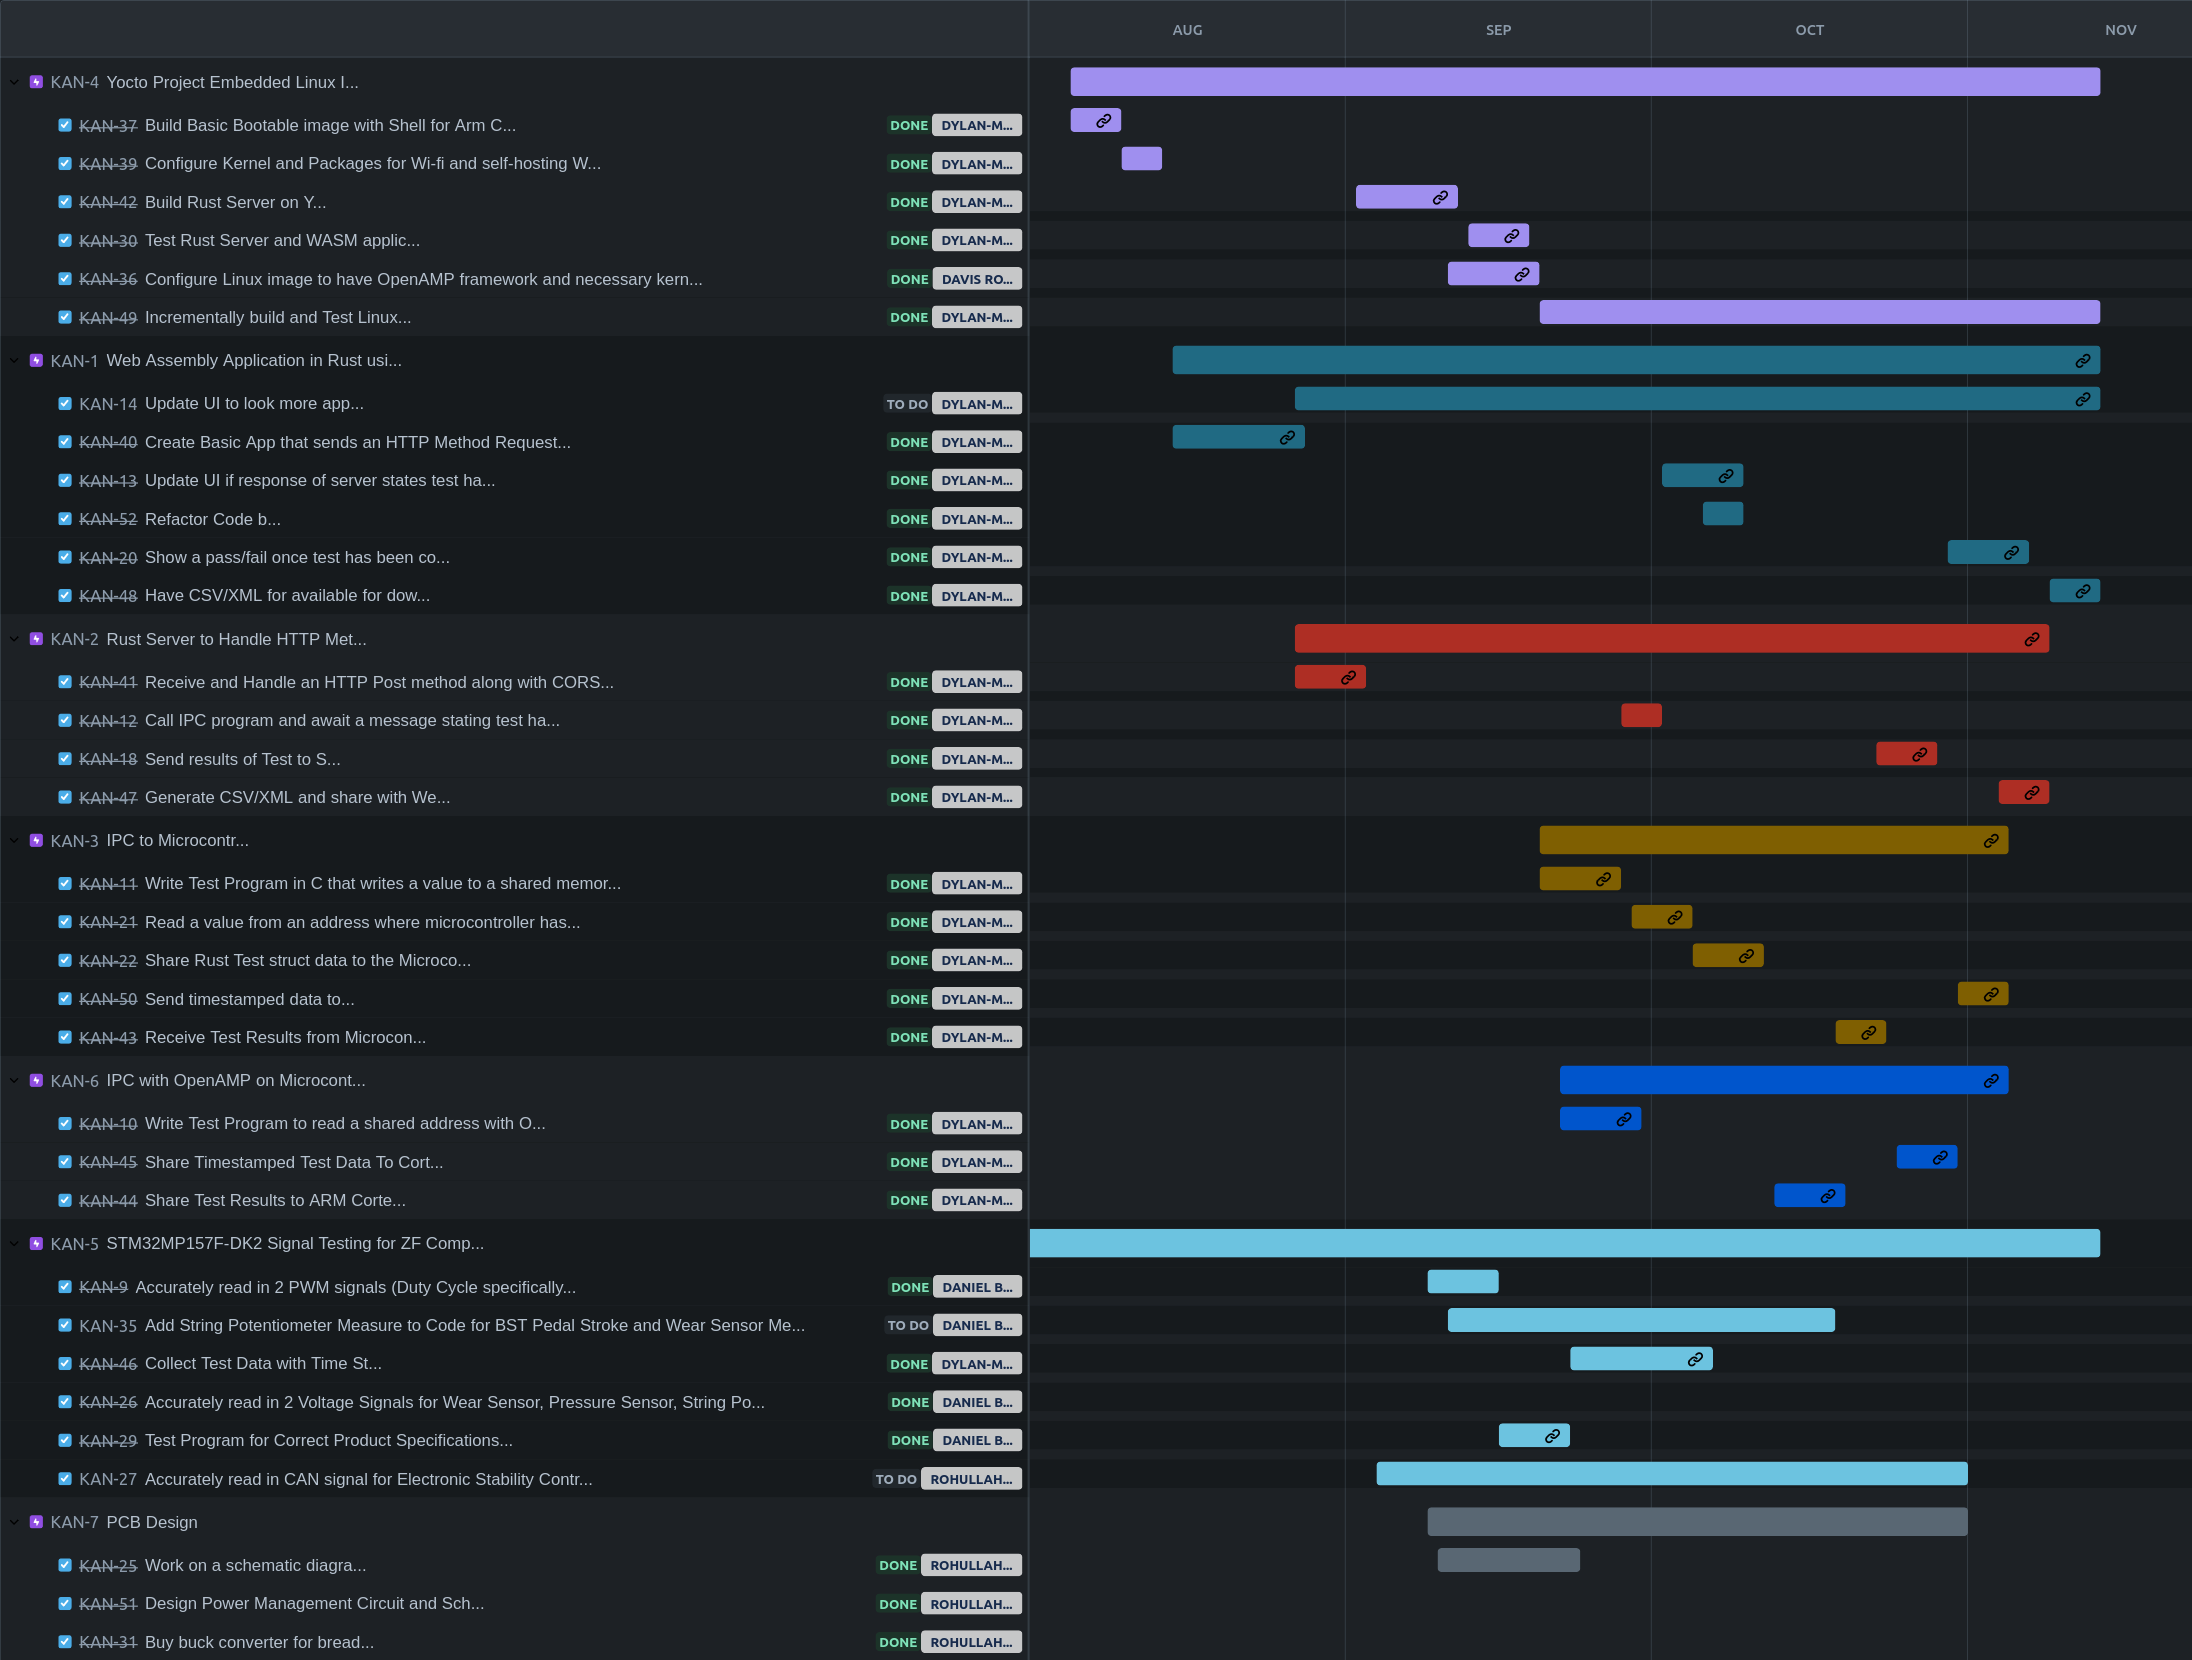
\includegraphics[height=0.85\paperheight]{assets/diagrams/gantt.png}
\end{frame}

%==============================================================================
% DESIGN AND IMPLEMENTATION SECTION: Budget Projection
%==============================================================================
\begin{frame}
  \frametitle{Budget Projection}
  \centering
  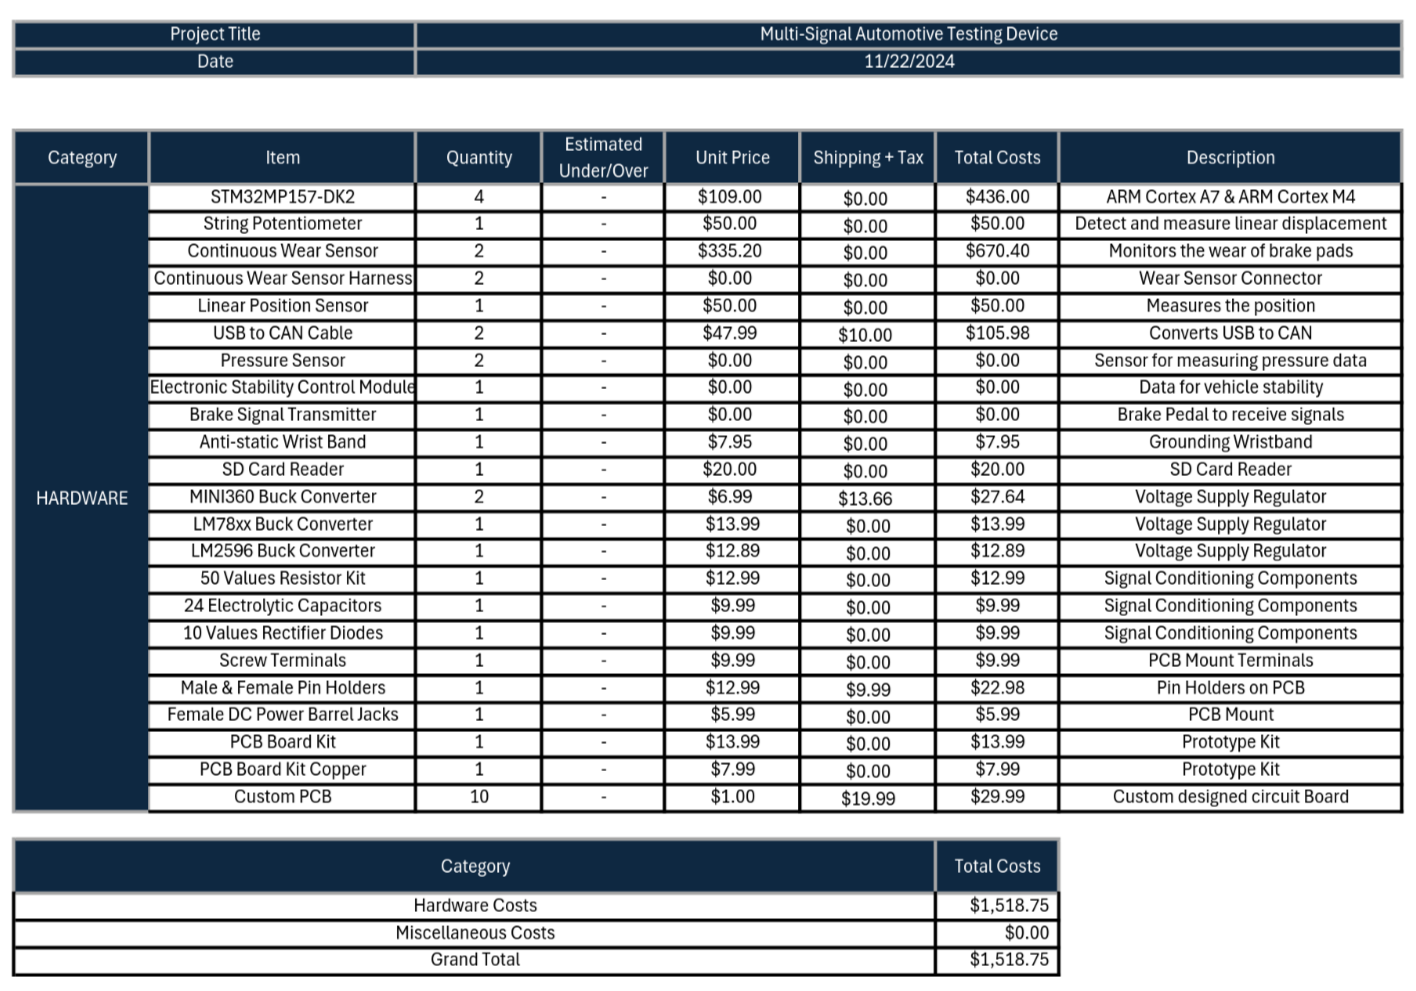
\includegraphics[height=0.80\paperheight]{assets/diagrams/budget.png}
\end{frame}

\AtBeginSubsection[]
{
  \begin{frame}
    \frametitle{Table of Contents}
    \tableofcontents[currentsubsection]
  \end{frame}
}

%==============================================================================
% DESIGN AND IMPLEMENTATION SECTION: Hardware Design
%==============================================================================
\subsection{Hardware Design}
\begin{frame}
  \frametitle{Power Supply Schematic Design}
  \begin{minipage}{0.7\textwidth}
    \begin{figure}
      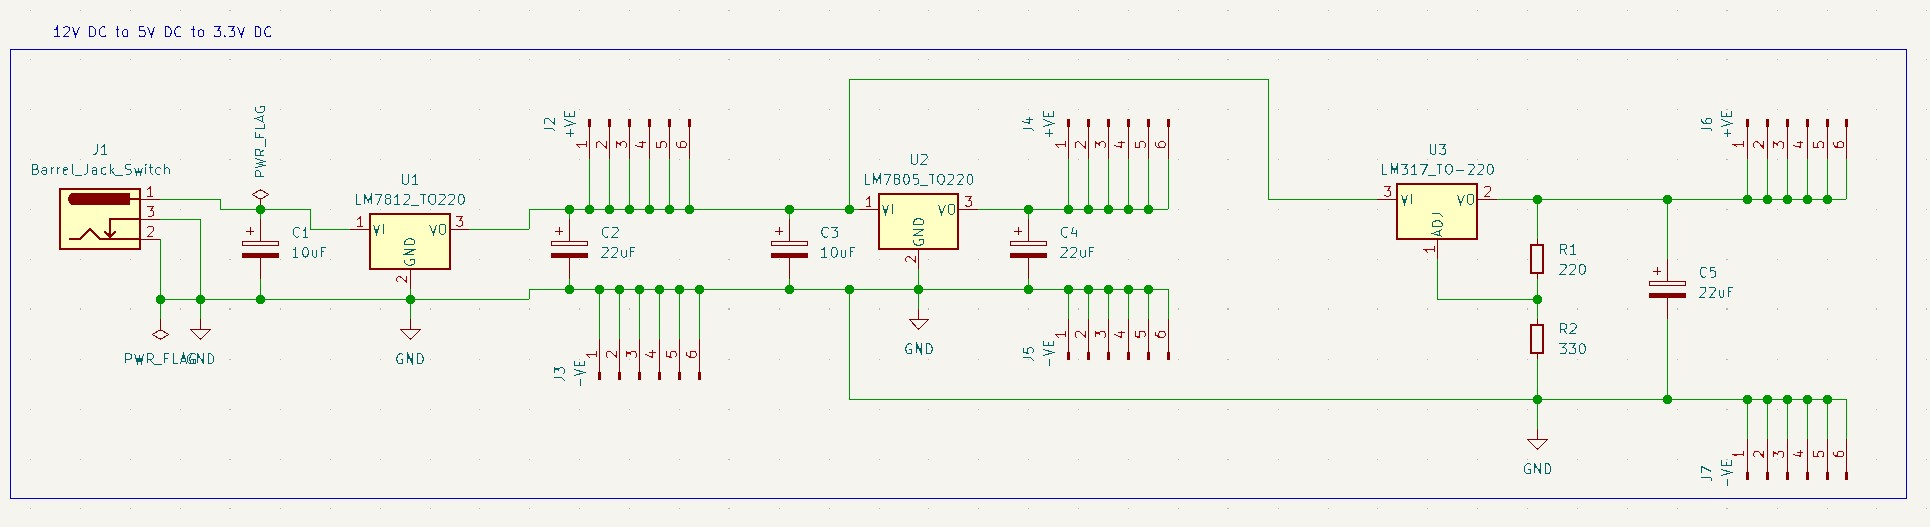
\includegraphics[width=\textwidth]{assets/electronic/pwrsupply.jpg}
      \caption{\it power management system that converts 12V DC input into multiple usable voltage levels.}
    \end{figure}
  \end{minipage}
  \hfill
  \begin{minipage}{0.275\textwidth}
    \begin{block}{Overview}
      \begin{itemize}
          \small
        \item 12V DC stable voltage using LM7812 (1A)
        \item 12V to 5V DC using LM7805 (1A)
        \item 12V to 3.3V using LM317 adjustable regulator
      \end{itemize}
    \end{block}
    \begin{block}{Key Components}
      \begin{itemize}
          \small
        \item LM7812, LM7805, LM317 voltage regulators for step-down conversion.
        \item Capacitors for noise filtration.
        \item Resistors to set voltages for LM317 as 3.146V DC (50uA).
      \end{itemize}
    \end{block}
  \end{minipage}
\end{frame}

\begin{frame}
  \frametitle{Schematic Design - Brake Signal Transmitter}
  \begin{minipage}{0.6\textwidth}
    \begin{figure}
      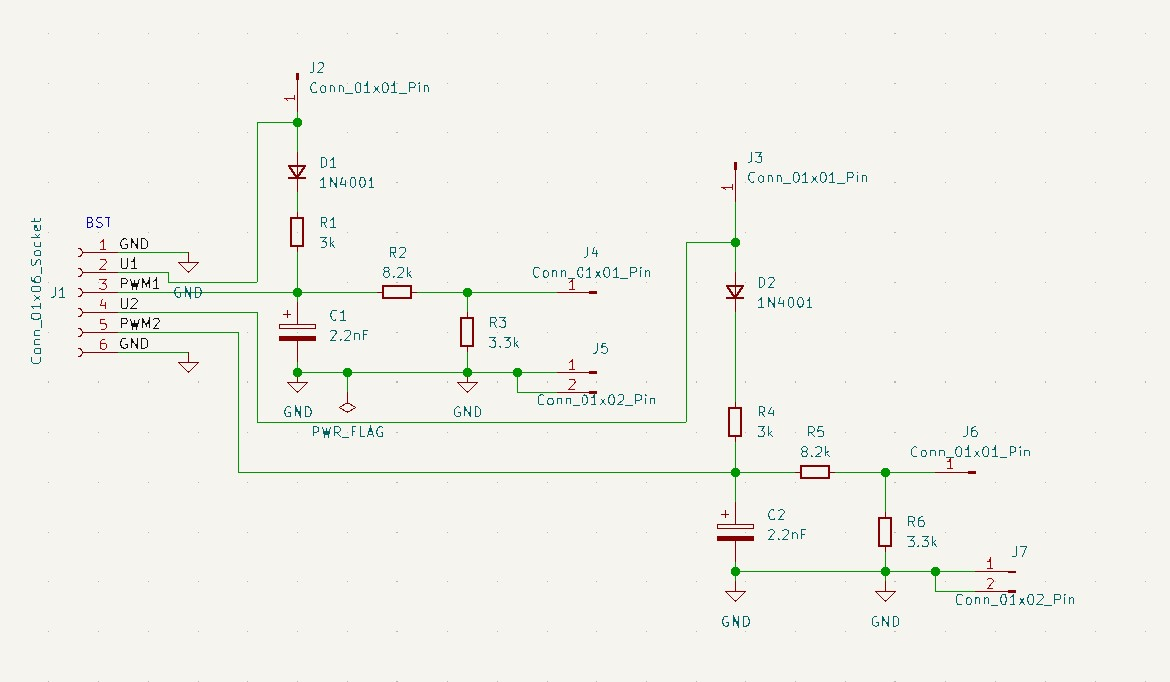
\includegraphics[width=\textwidth]{assets/electronic/bst_schem.jpg}
      \caption{Circuit schematic of Brake Signal Transmitter (BST)}
    \end{figure}
  \end{minipage}
  \hfill
  \begin{minipage}{0.375\textwidth}
    \begin{block}{Key Points}
      \begin{itemize}
        \item Captures the output of the Brake Signal Transmitter (BST) in the form of Pulse Width Modulation (PWM) signals.
        \item Includes resistors and capacitors for signal filtering.
        \item Diodes protect the circuit from voltage surges and reverse polarity.
      \end{itemize}
    \end{block}
  \end{minipage}
\end{frame}

\begin{frame}
  \frametitle{Peripheral Interface Schematic Diagram }
  \begin{minipage}{0.495\textwidth}
    \begin{figure}
      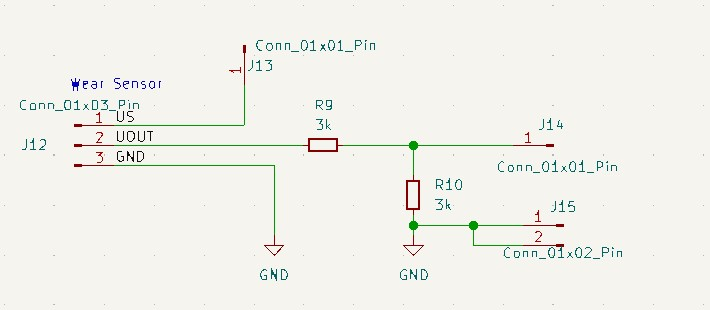
\includegraphics[width=\textwidth]{assets/electronic/wear_schem.jpg}
      \caption{Continuous Wear Sensor Interface Schematic}
    \end{figure}
    \begin{figure}
      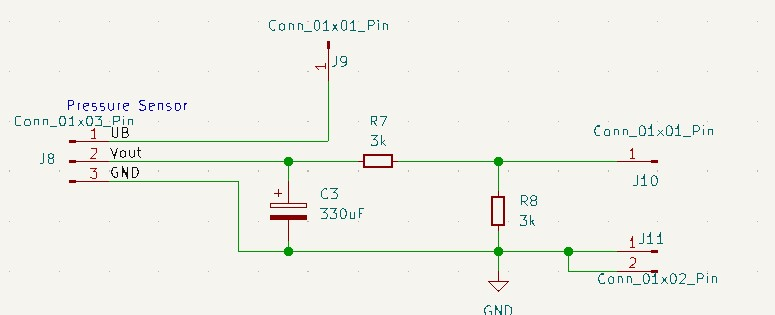
\includegraphics[width=\textwidth]{assets/electronic/pressure_schem.jpg}
      \caption{Pressure Sensor Interface Schematic}
    \end{figure}
  \end{minipage}
  \hfill
  \begin{minipage}{0.49\textwidth}
    \begin{figure}
      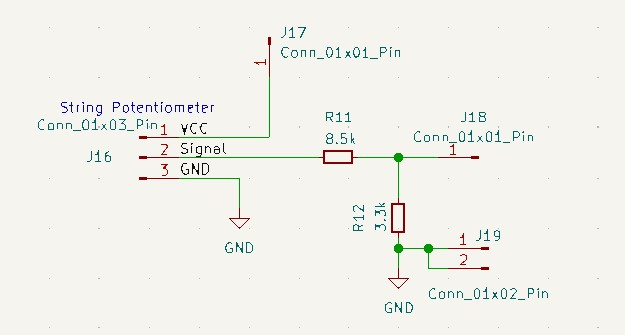
\includegraphics[width=\textwidth]{assets/electronic/string_pcb.jpg}
      \caption{String Potentiometer Interface Schematic}
    \end{figure}

    \vspace{-0.5cm}
    \begin{block}{Key Points}
      \begin{itemize}
        \item Captures analog voltage signals to monitor brake wear and pressure sensor and displacement on the string potentiometer.
        \item Uses voltage dividers for safe microcontroller input levels.
        \item Uses capacitors to stabilize the output.
      \end{itemize}
    \end{block}
  \end{minipage}
\end{frame}
\begin{frame}
  \frametitle{Printed Circuit Board Design}
  \begin{minipage}{0.3\textwidth}
    \begin{figure}
      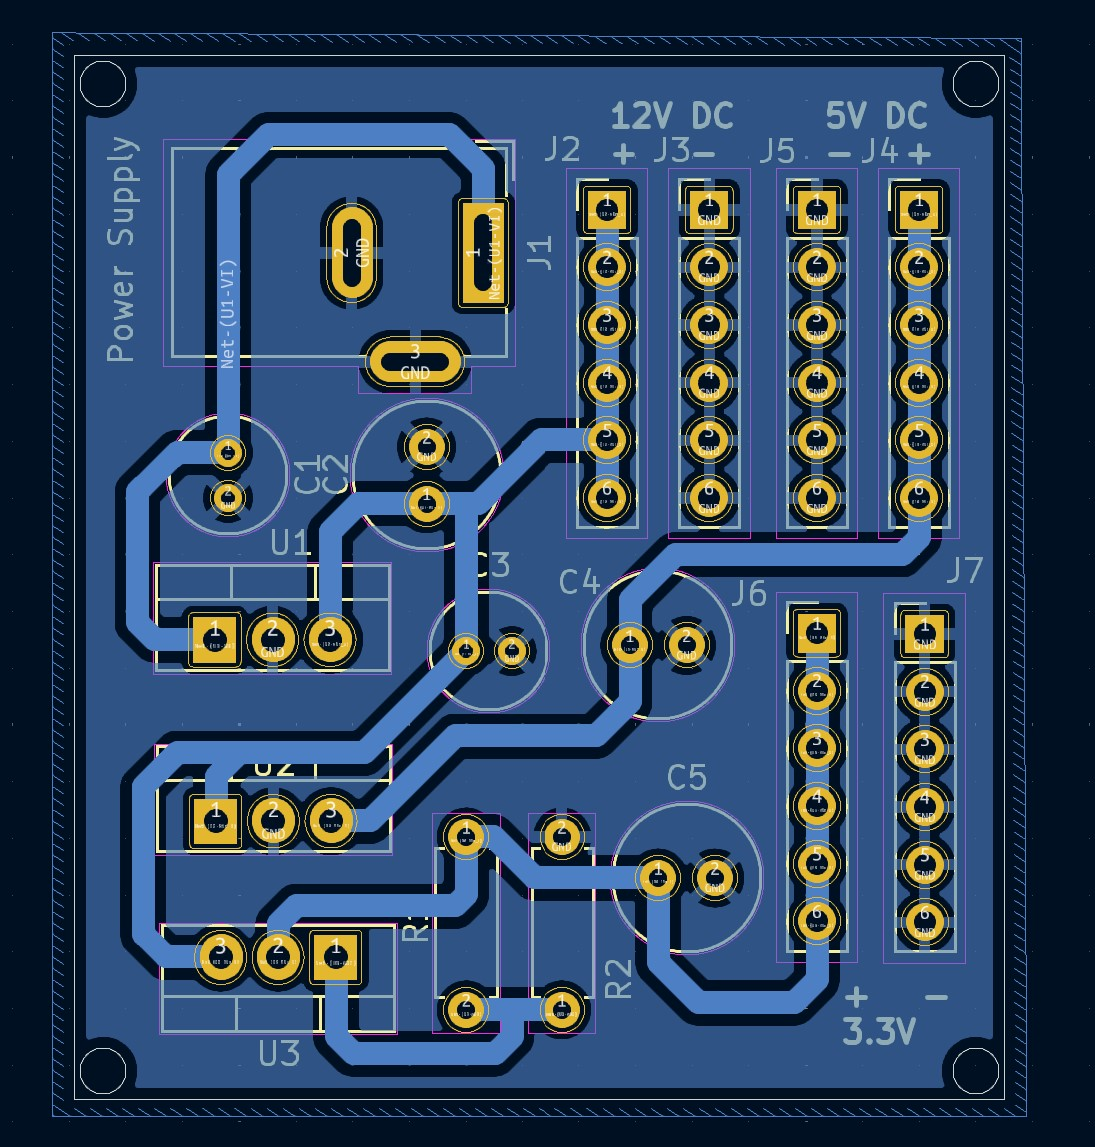
\includegraphics[width=\textwidth]{assets/electronic/pwrsupply_pcb.jpg}
      \caption{PCB for Power Management}
    \end{figure}
  \end{minipage}
  \hfill
  \begin{minipage}{0.675\textwidth}
    \begin{block}{Overview}
      \begin{itemize}
          \small
        \item The power supply PCB converts the 12V DC input from the DC jack into regulated output voltages for the system.
          \begin{itemize}
              \tiny
            \item  12V DC
            \item 5V DC
            \item 3.3V DC
          \end{itemize}
        \item It is designed based on the schematic with components such as voltage regulators (LM7812, LM7805, LM317), capacitors, and resistors.
      \end{itemize}
    \end{block}
    \begin{block}{Key Components}
      \begin{itemize}
          \footnotesize
        \item DC Jack (J1): Connects the input 12V DC power supply to the board.
        \item Output Pins:
          \begin{itemize}
              \tiny
            \item J2/J3: Provides 12V DC output.
            \item J4/J5: Provides 5V DC output.
            \item J6/J7: Provides 3.3V DC output.
          \end{itemize}
        \item Voltage Regulators
          \begin{itemize}
              \tiny
            \item Step-down conversion for different voltage levels.
            \item Smooth and stable output.
          \end{itemize}
        \item Capacitors (C1-C5)
          \begin{itemize}
              \tiny
            \item Ensure smooth voltage output by filtering noise and ripples.
          \end{itemize}
        \item Ground connections: All components are referenced to a common ground for stable operation.
      \end{itemize}
    \end{block}
  \end{minipage}
\end{frame}

\begin{frame}
  \frametitle{Peripherals Printed Circuit Board}
  \begin{minipage}{0.5\textwidth}
    \begin{block}{Key Features}
      \begin{itemize}
          \small
        \item Input/Power Pins:
          \begin{itemize}
              \footnotesize
            \item Each DUT has a dedicated connector for input signals and a power signal.
            \item J1: Inputs for BST (PWM1 and PWM2) | J2/J3: 12V Power Signals for BST (PWM1 and PWM2)
            \item J8: Pressure sensor input | J9: 12V DC Power Signal
            \item J12: Wear sensor input | J13: 5V DC Power Signal
            \item J16: String Potentiometer input | J17: 12V DC Power signal
          \end{itemize}
        \item Output Pins:
          \begin{itemize}
              \footnotesize
            \item Processed signals are sent to the microcontroller through the output pins.
            \item J4/J5/J6/J7: BST processed signals
            \item J10/J11: Pressure sensor output
            \item J14/J15: Wear sensor output
            \item J18/J19: String potentiometer output.
          \end{itemize}
        \item Signal Conditioning:
          \begin{itemize}
              \footnotesize
            \item Resistors: Scale signals for safe microcontroller input.
            \item Capacitors: Filter noise and stabilize signals.
            \item Capacitors: Filter noise and stabilize signals.
          \end{itemize}
      \end{itemize}
    \end{block}
  \end{minipage}
  \hfill
  \begin{minipage}{0.45\textwidth}
    \begin{figure}
      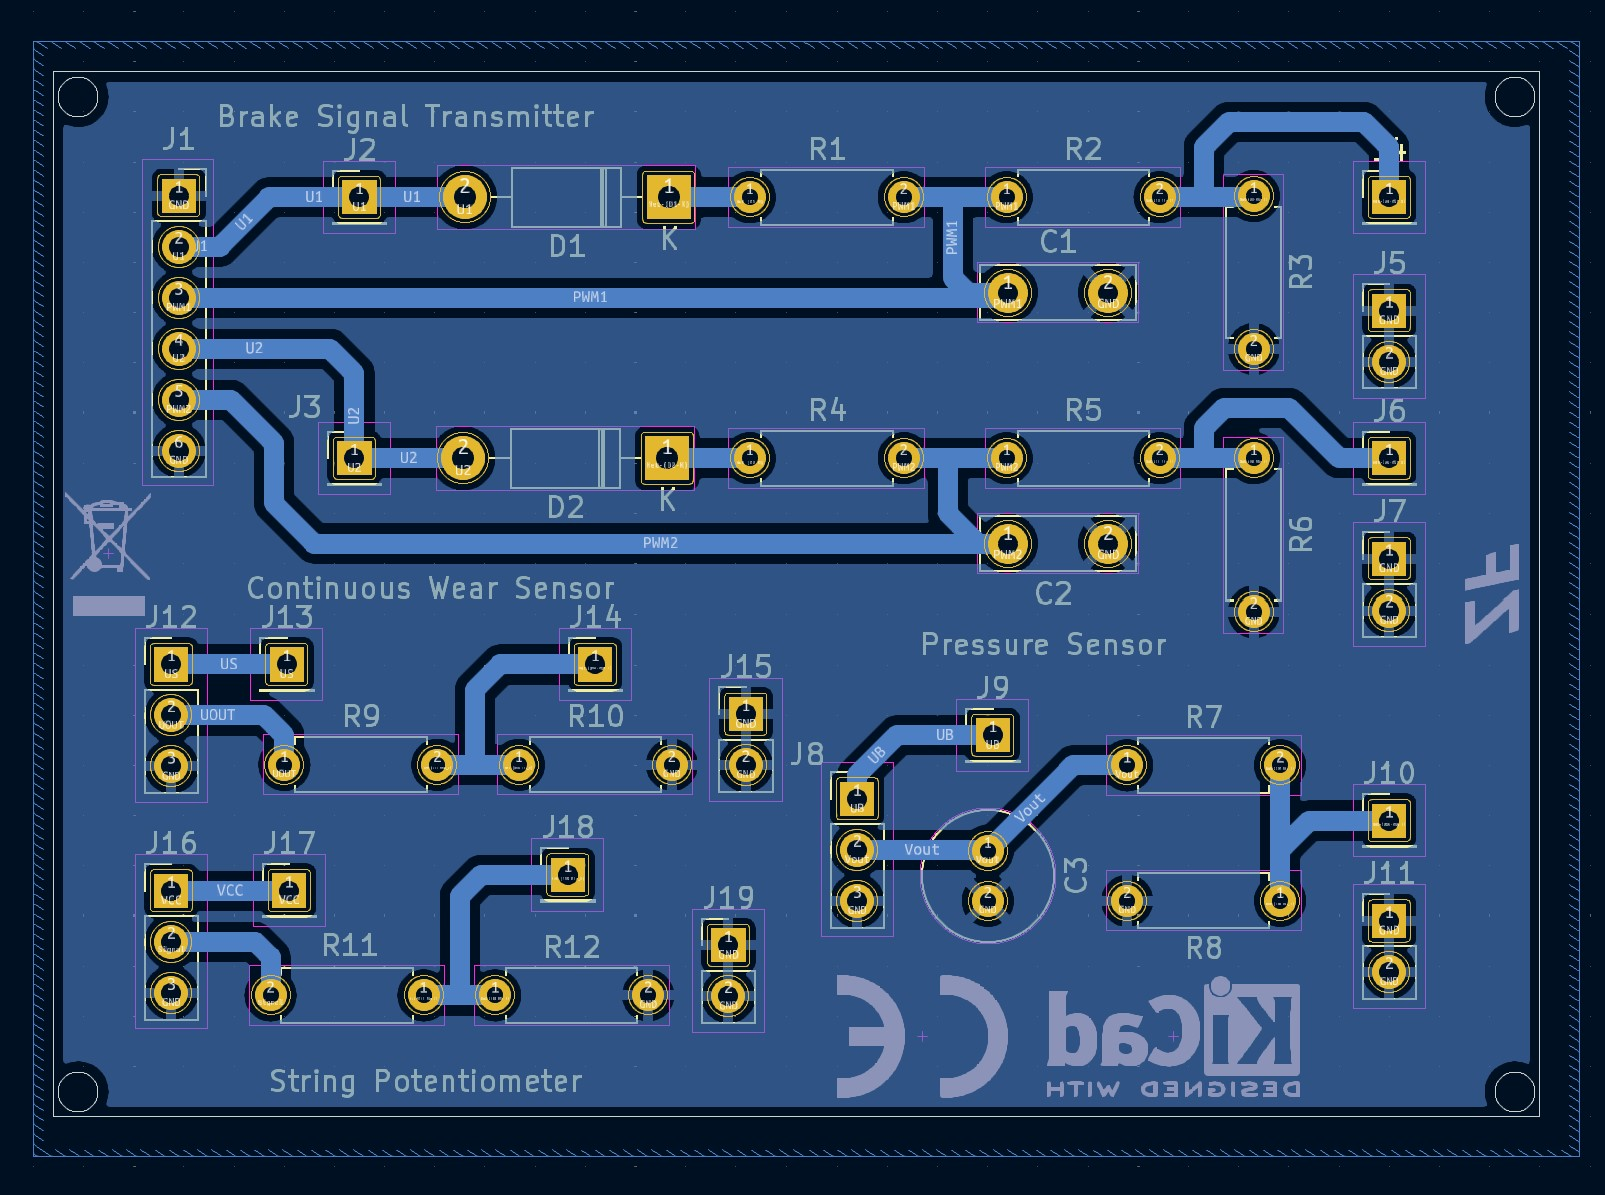
\includegraphics[width=\textwidth]{assets/electronic/peri_pcb.jpg}
      \caption{PCB for connecting to peripheral device}
    \end{figure}
  \end{minipage}
\end{frame}

\begin{frame}
  \frametitle{Fabricated PCB}
  \begin{minipage}{0.5\textwidth}
    \begin{figure}
      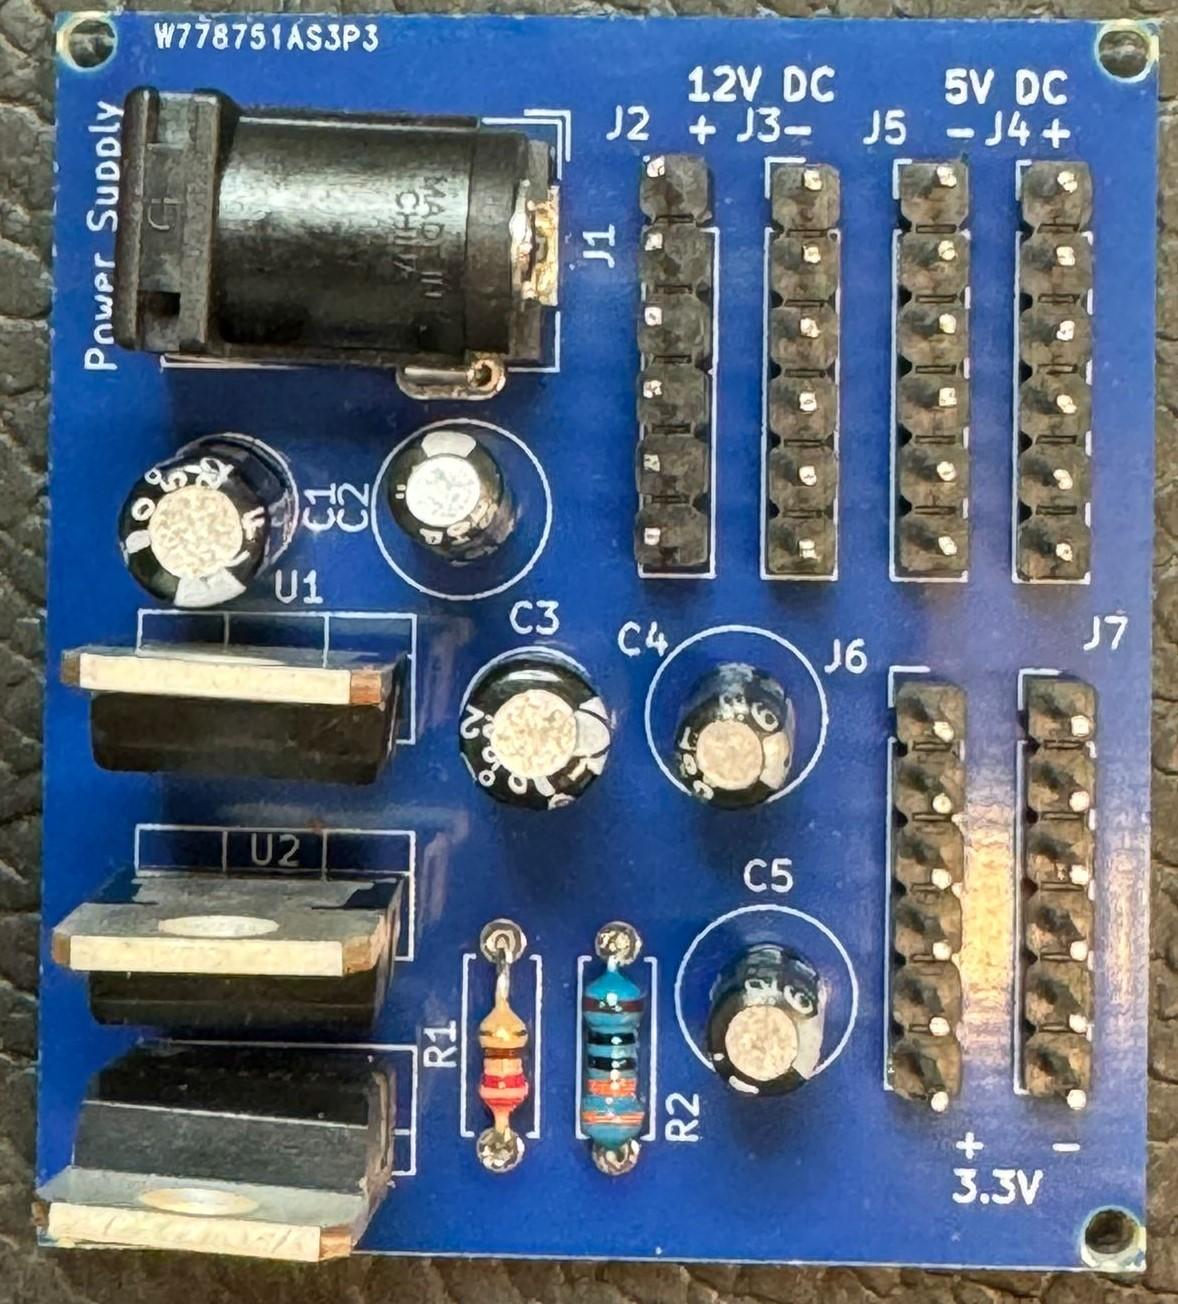
\includegraphics[width=0.9\textwidth]{assets/electronic/pcb1.jpeg}
      \caption{Power Management PCB}
    \end{figure}
  \end{minipage}
  \hfill
  \begin{minipage}{.475\textwidth}
  \begin{figure}
    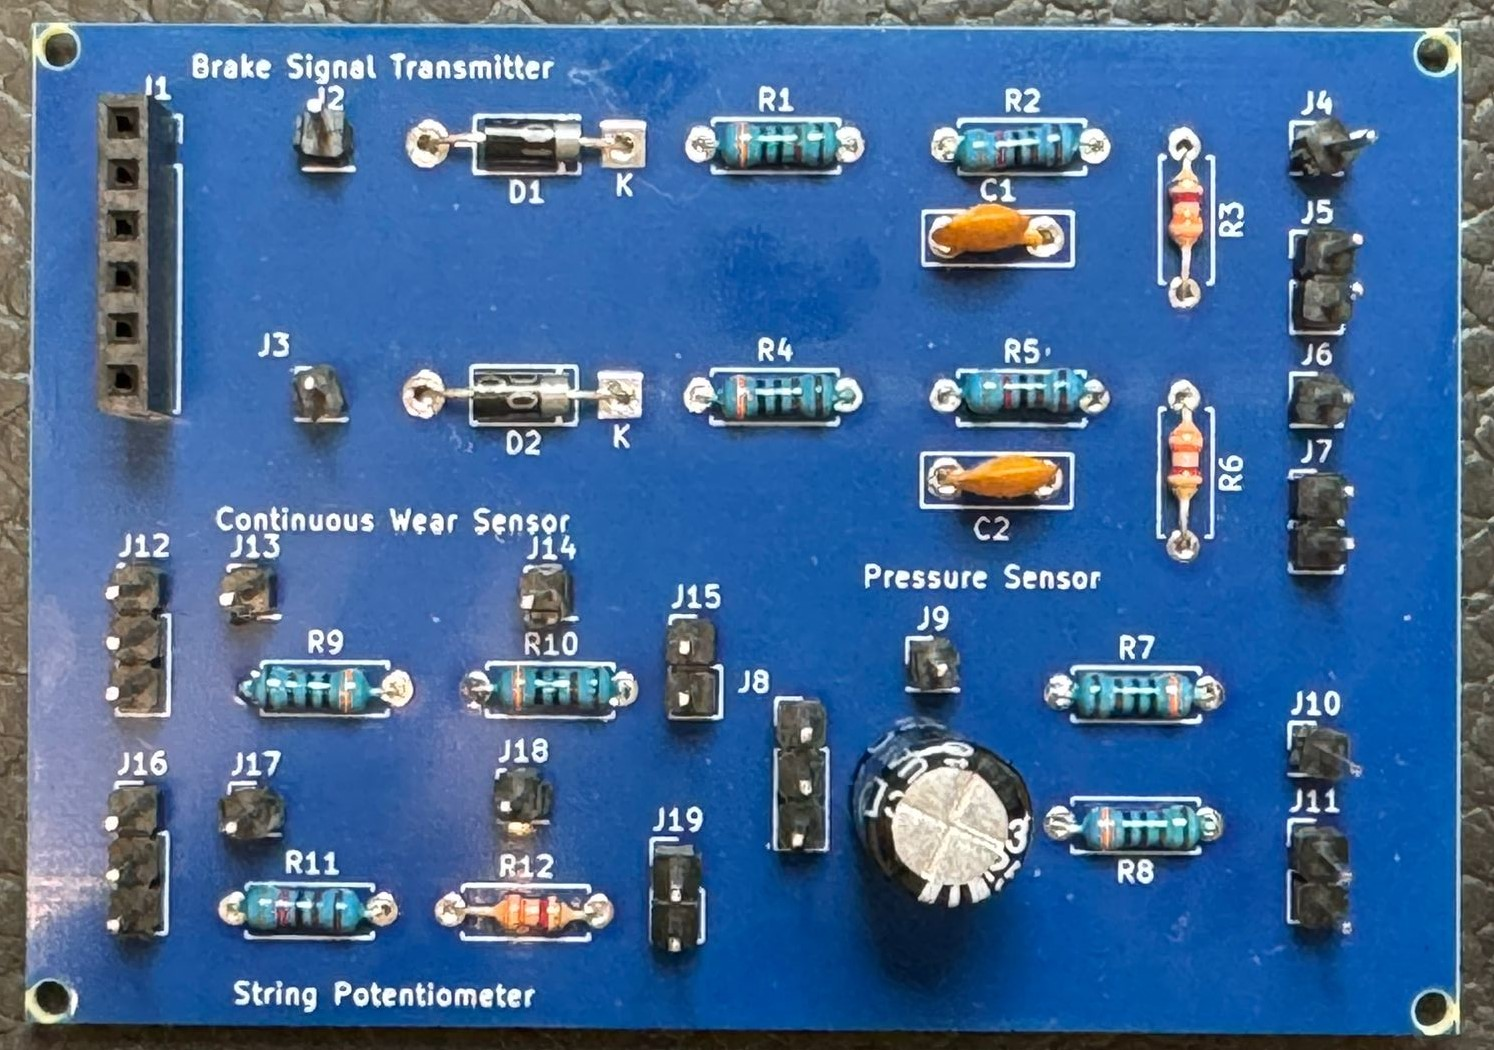
\includegraphics[width=\textwidth]{assets/electronic/pcb2.jpeg}
      \caption{Peripheral Interface PCB}
  \end{figure}
  \end{minipage}
\end{frame}

\begin{frame}
  \frametitle{Enclosure Design}
  \begin{minipage}{0.475\textwidth}
    \begin{figure}
      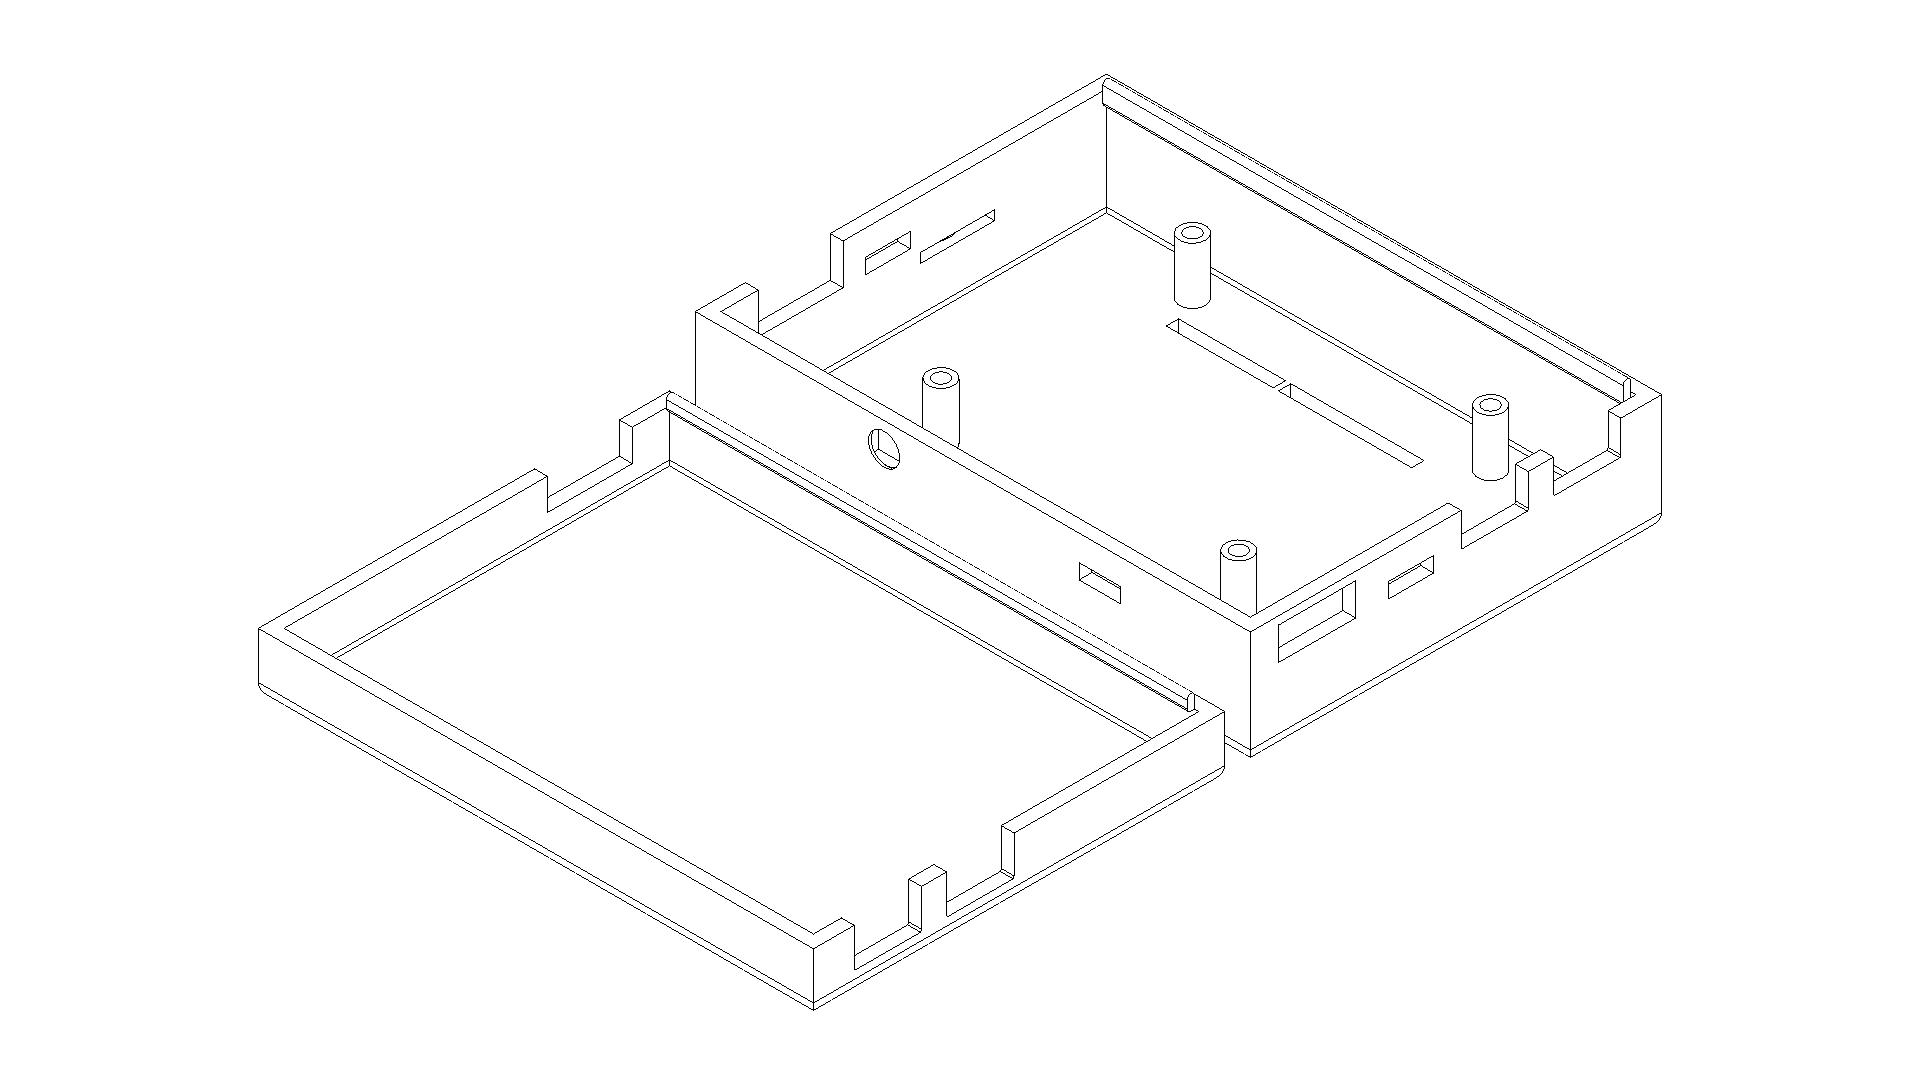
\includegraphics[width=0.95\textwidth]{assets/electronic/stm32_enclosure_final_test_pic1.jpg}
      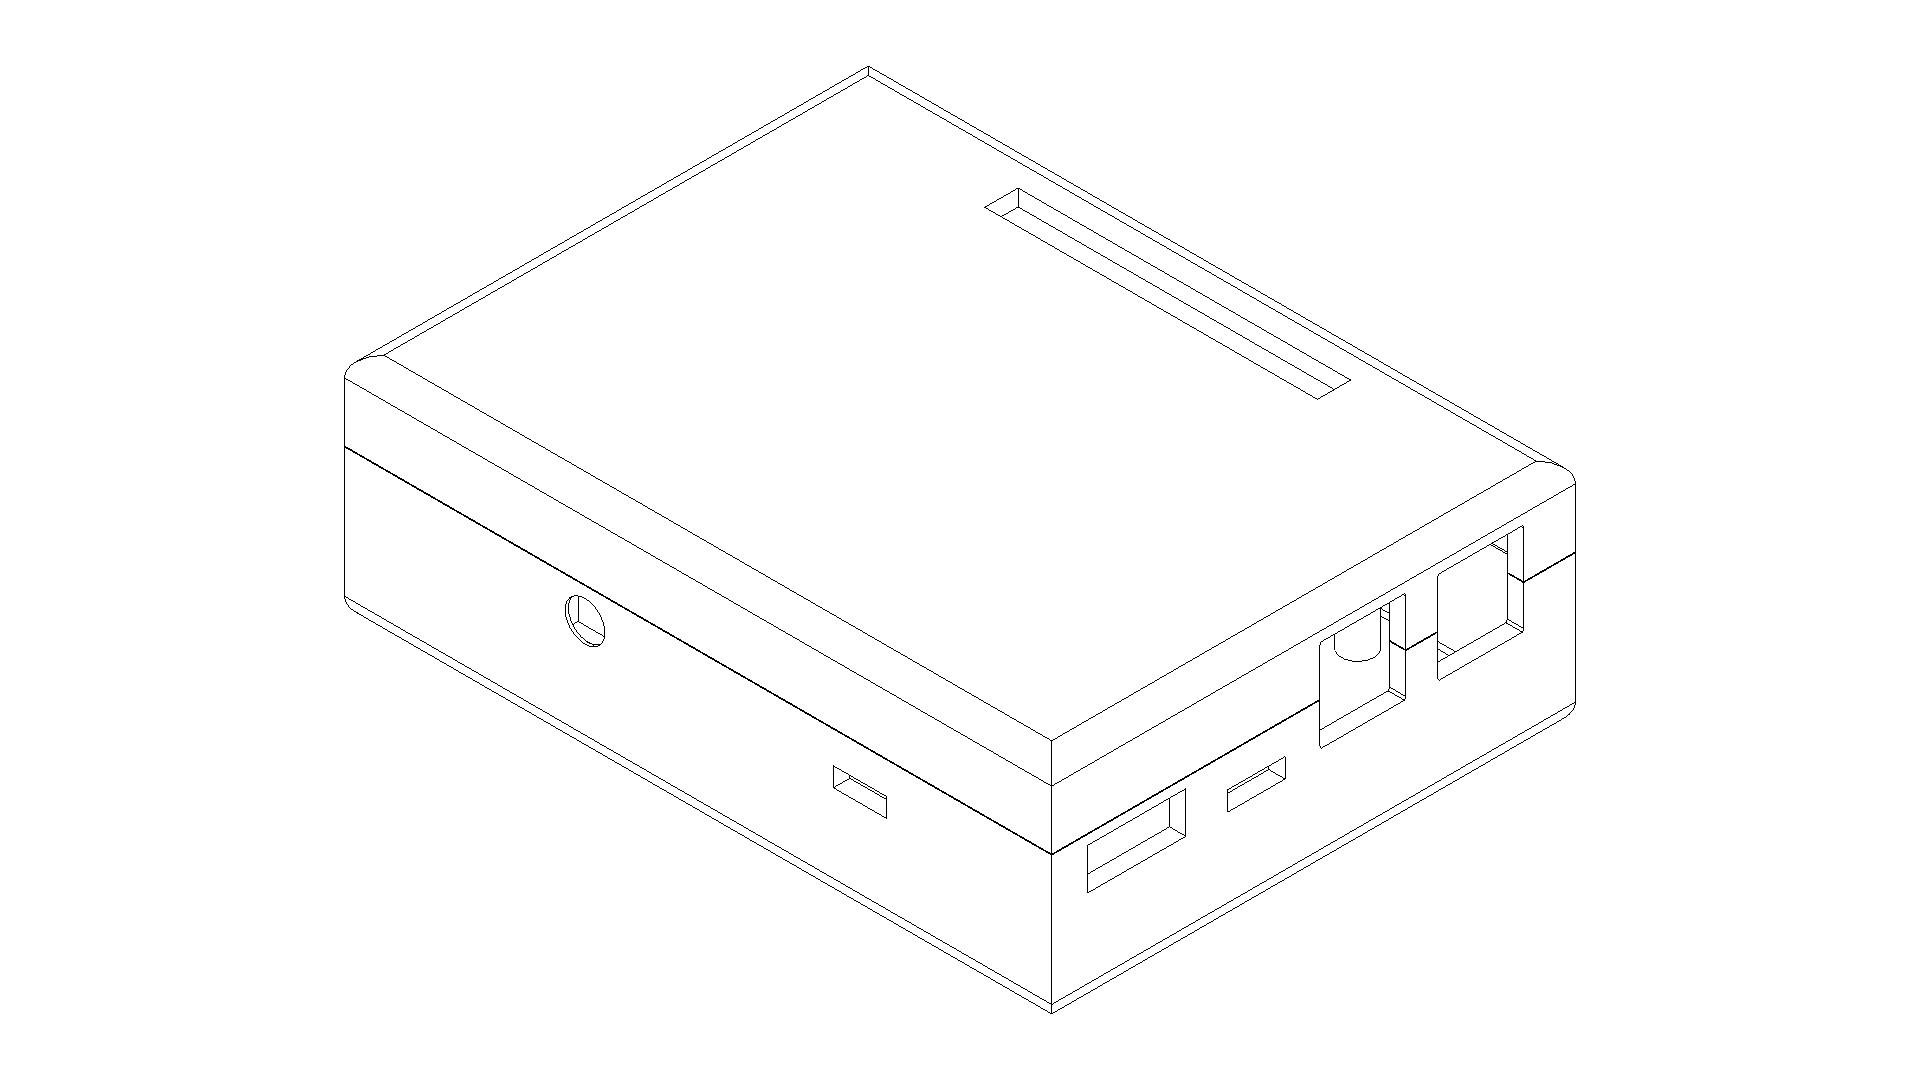
\includegraphics[width=0.95\textwidth]{assets/electronic/stm32_enclosure_final_testpic2.jpg}
      \caption{\it Enclosure for STM32MP157F-DK2}
    \end{figure}
  \end{minipage}
  \hfill
  \begin{minipage}{0.45\textwidth}
    \begin{figure}
      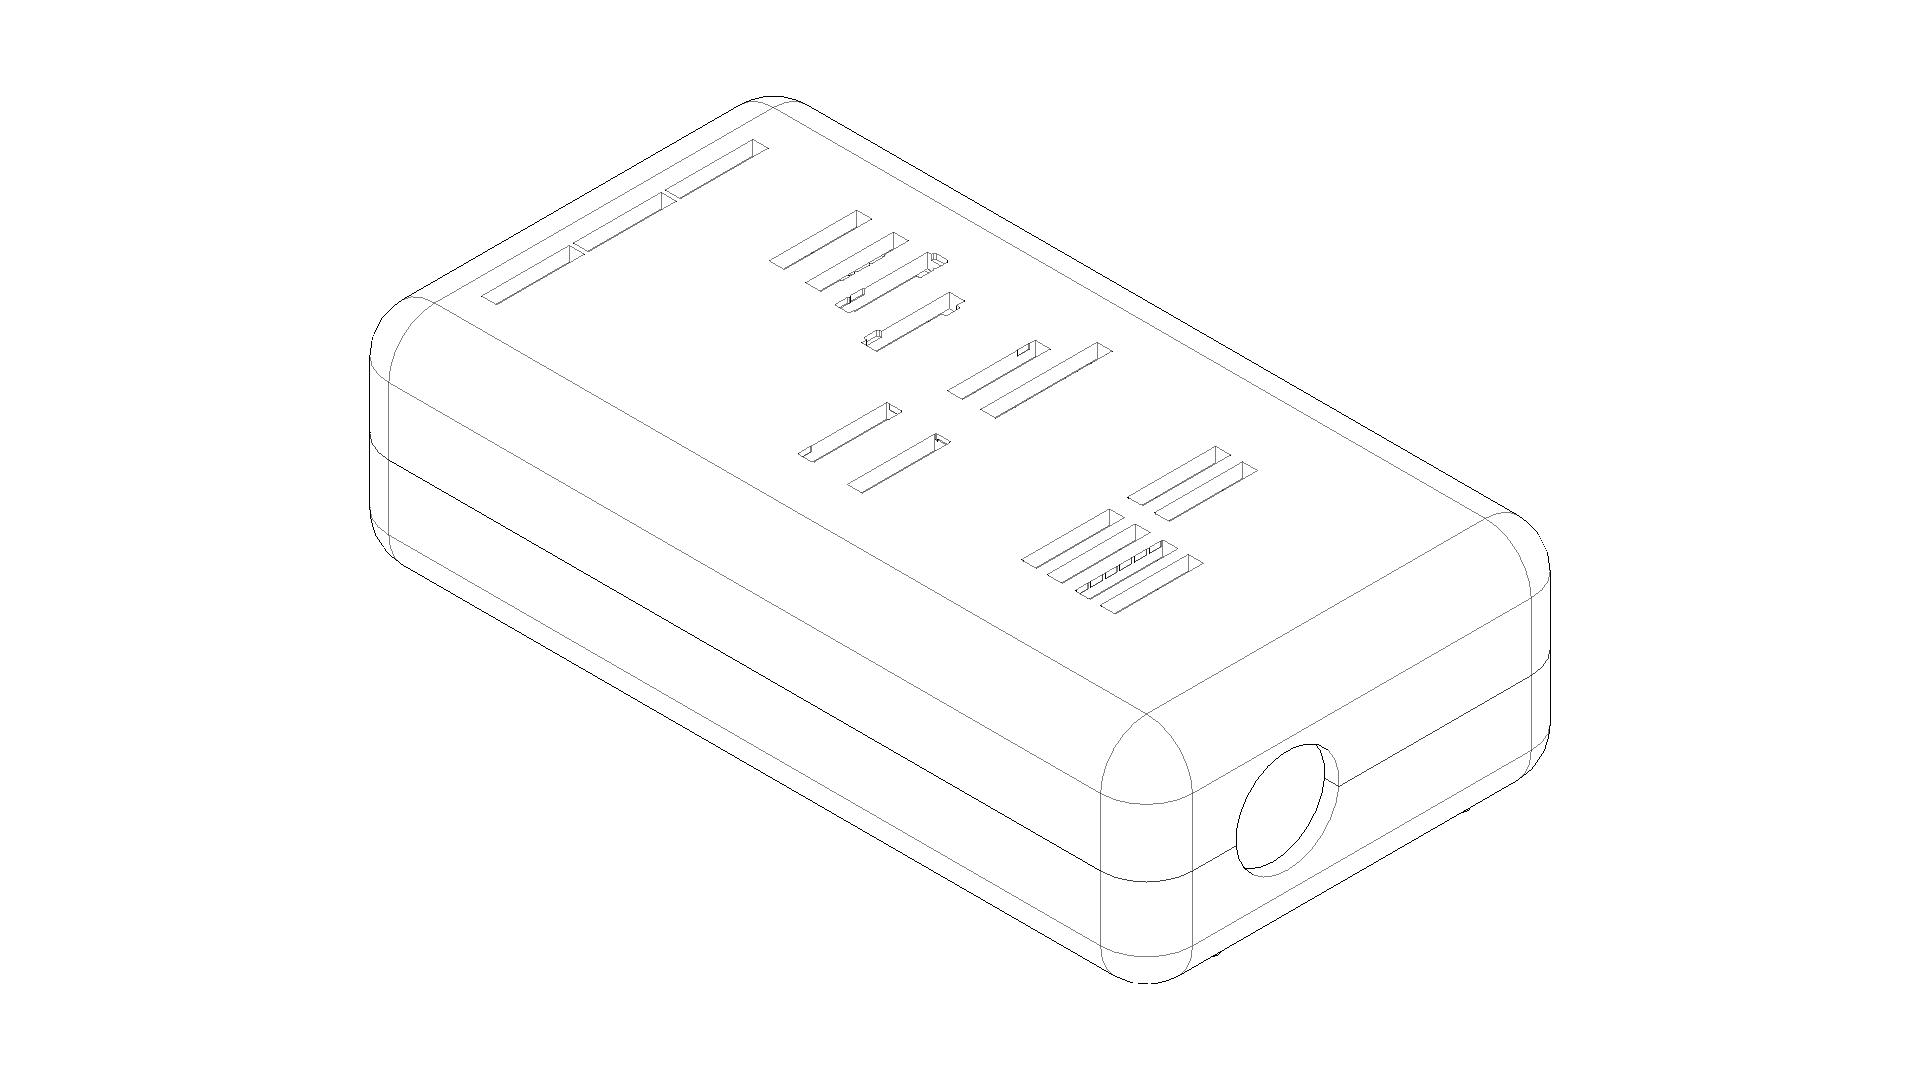
\includegraphics[width=0.95\textwidth]{assets/electronic/psperi_enclosure_final_testpic1.jpg}
      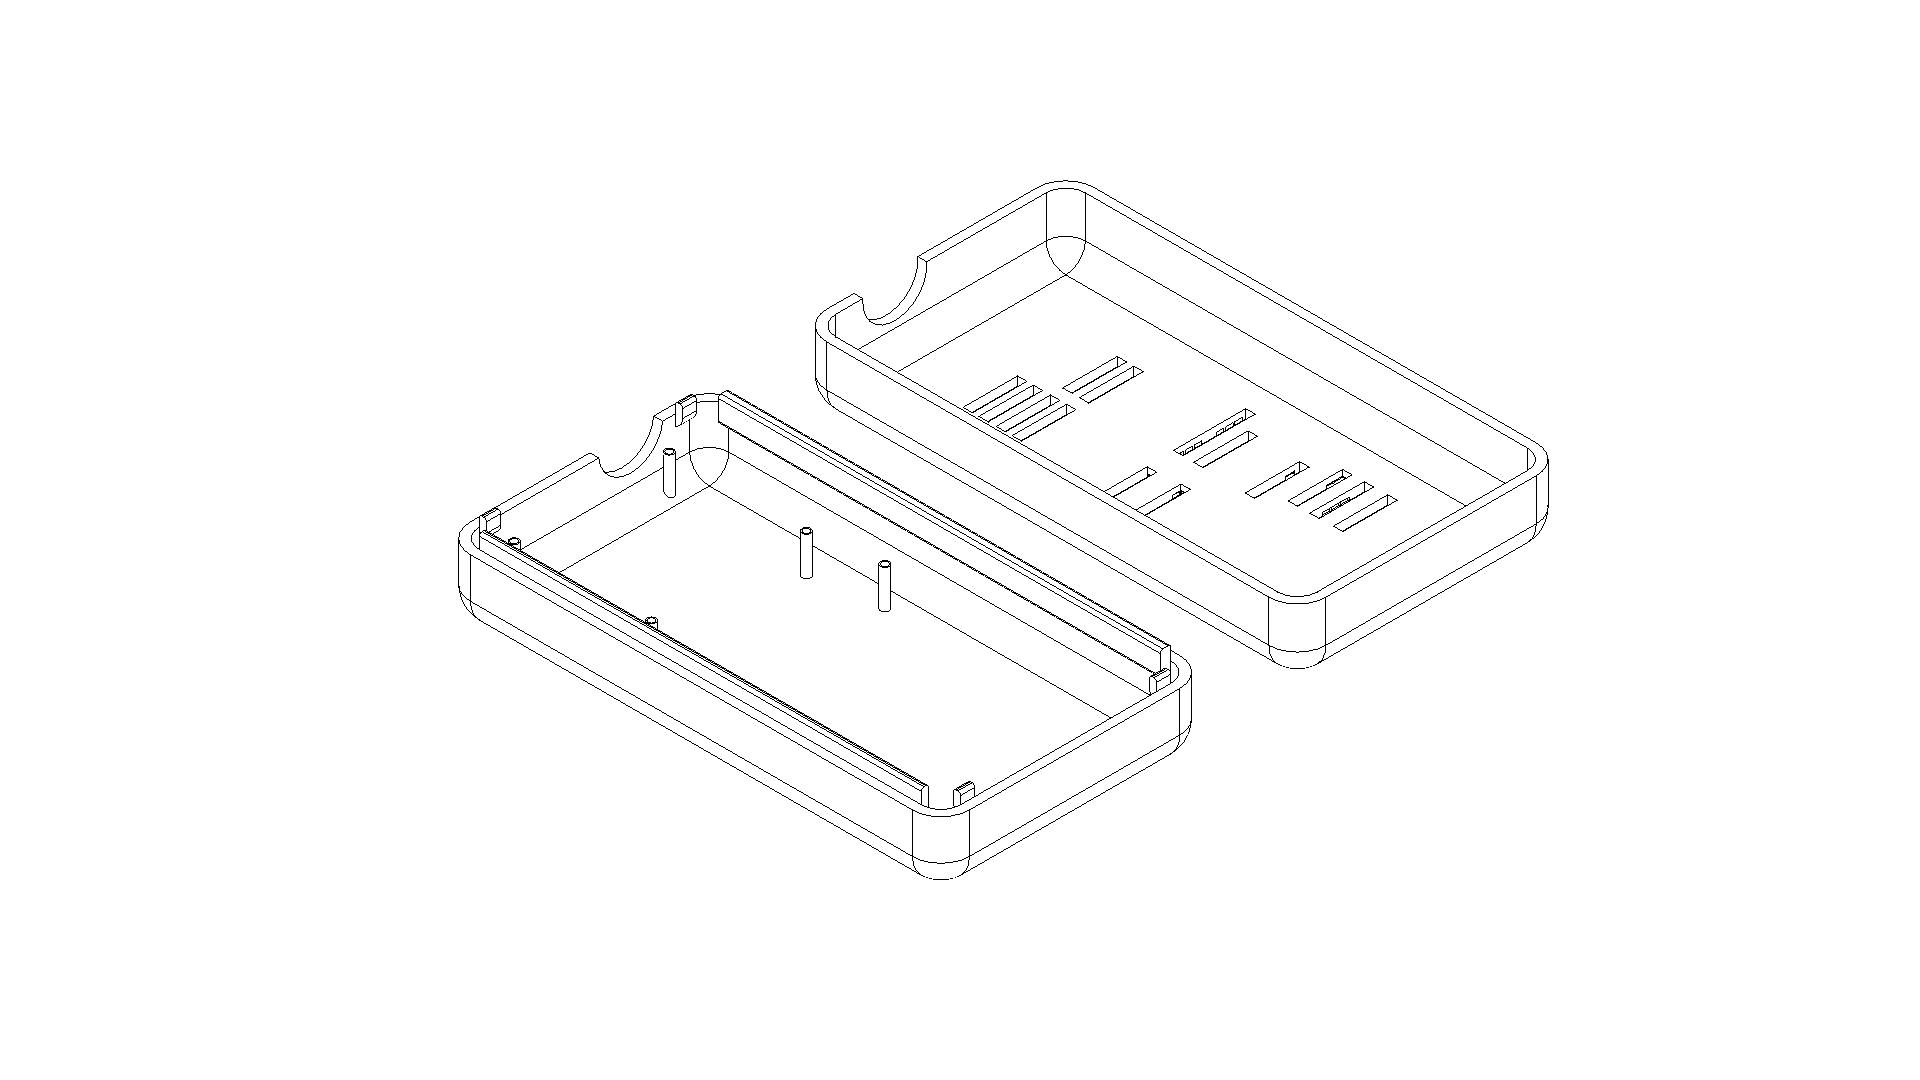
\includegraphics[width=0.95\textwidth]{assets/electronic/psperi_enclosure_final_testpic2.jpg}
      \caption{\it Enclosure for PCBs}
    \end{figure}
  \end{minipage}
\end{frame}

%==============================================================================
% DESIGN AND IMPLEMENTATION SECTION: Cortex-M4 Firmware
%==============================================================================
\subsection{Device Interfacing and Testing}
\begin{frame}
  \frametitle{Firmware to Test Brake Signal Transmitter (BST)}
  \begin{block}{Purpose}
    \small{
      \begin{itemize}
        \item Developed firmware on the onboard Cortex-M4 microcontroller to validate BST
        \item Ensures brake actuation is accurate to distance moved by brake pedal
        \item \LightBold{Key Specifications:} Output range 1 mm to 9 mm, Sensitivity 5.96\% DC/mm, Output signals PWM1 and PWM2 (S1 and S2)
      \end{itemize}
    }
  \end{block}
  \hspace{-0.5cm}
  \begin{minipage}{0.485\textwidth}
    \begin{block}{Method}
      \small{
        \begin{itemize}
          \item \LightBold{Input Capture:} Timers captures read two PWM signals from the BST
          \item \LightBold{ADC Reading:}Optional string potentiometer for direct analog voltage measurements via ADC 
          \item \LightBold{Processing:} Calculates duty cycles, frequencies, and estimated stroke via timer interrupts
          \item \LightBold{Validation:} Compare measurements against expected values according to product specifications to verify BST accuracy
          \item \LightBold{Results:} Sends test results to the main processor for logging and user display
        \end{itemize}
      }
    \end{block}
  \end{minipage}
  \hfill
  \begin{minipage}{0.50\textwidth}
    \begin{figure}
      \centering
      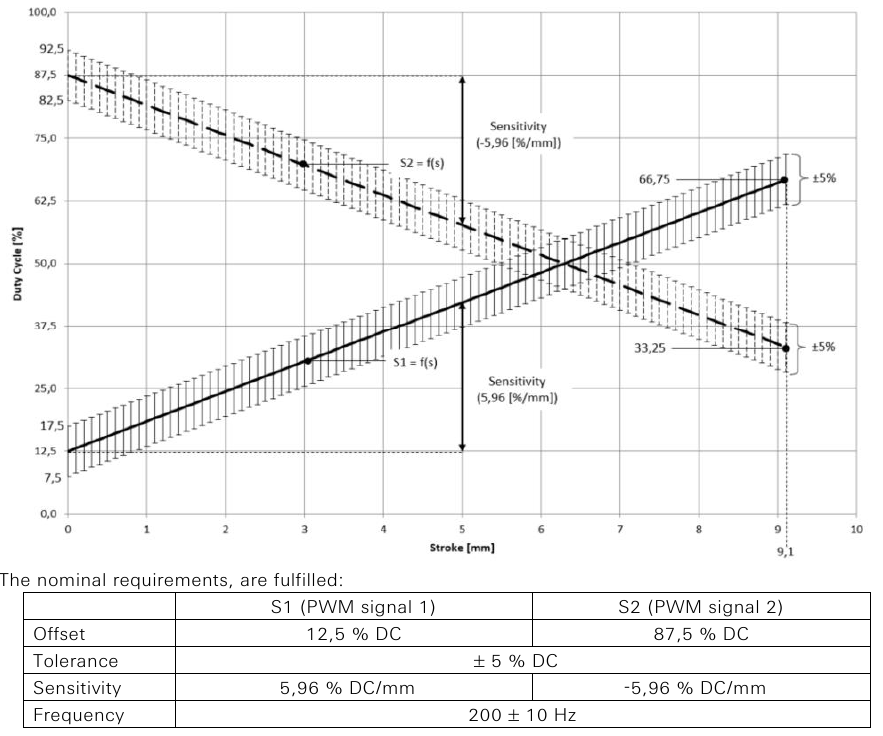
\includegraphics[width=0.85\textwidth]{assets/specs/bst_product_specs.png}
      \caption{\it Product Specifications for BST}
    \end{figure}
  \end{minipage}
\end{frame}

% CWS Test implementation
\begin{frame}
    \frametitle{Firmware to Test Continuous Wear Sensor (CWS)}
    \begin{block}{Purpose}
        \small{
            \begin{itemize}
                \item Developed firmware on the onboard Cortex-M4 microcontroller to validate the Continuous Wear Sensor (CWS)
                \item Ensures accurate measurement of brake pad wear levels to enhance vehicle safety
                \item \LightBold{Key Specifications:} Output range 0.7V (18 mm or new pad) to 4.0 V (53 mm or worn pad), Sensitivity 0.08 V/mm, Voltage divider ratio 2:1
            \end{itemize}
        }
    \end{block}
    \hspace{-0.5cm}
    \begin{minipage}{0.485\textwidth}
        \begin{block}{Method}
            \small{
                \begin{enumerate}
                    \tiny
                    \item \LightBold{ADC Configuration:} Read direct analog voltage via ADC using DMA for efficiency and a timer trigger for consistency
                    \item \LightBold{Wear Calculation:} Mapped the measured voltage to brake pad wear using a linear relationship and handled special conditions (e.g., new pad, worn-out pad) with specific tolerances
                    \item \LightBold{Validation:} Compared wear values against expected values based on product specifications
                    \item \LightBold{Results:} Error thresholds to determine pass/fail and send detailed test outcomes to the main processor for logging and user display
                \end{enumerate}
            }
        \end{block}
    \end{minipage}
    \hfill
    \begin{minipage}{0.50\textwidth}
        \begin{figure}
            \centering
            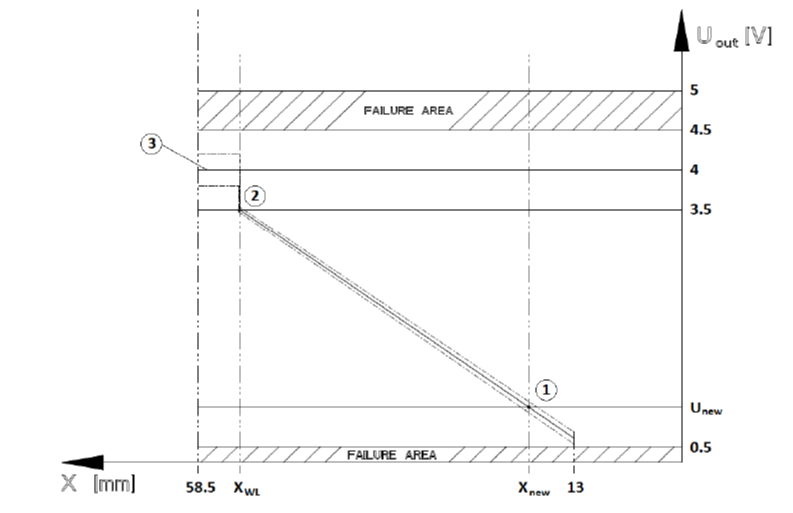
\includegraphics[width=\textwidth]{assets/specs/cws_product_specs.png}
            \caption{\it Product Specifications for CWS}
        \end{figure}
        \vspace{0.2cm}
    \end{minipage}
\end{frame}

% PS Test implementation
\begin{frame}
    \frametitle{Firmware to Test Pressure Sensor}
    \begin{block}{Purpose}
        \small{
            \begin{itemize}
                \item Developed firmware to validate Pressure Sensor readings on the Cortex-M4 microcontrooler
                \item Ensures accurate measurement of pressure when given for reliable vehicle control system purposes
                \item \LightBold{Key Specifications:} Output range 0.5V (0 bar) to 4.5 V (10 bar), Sensitivity 0.4 V/Bar, Voltage divider ratio 2:1
            \end{itemize}
        }
    \end{block}
    \hspace{-0.5cm}
    \begin{minipage}{0.485\textwidth}
        \begin{block}{Method}
            \small{
                \begin{enumerate}
                    \tiny
                    \item \LightBold{ADC Configuration:} Configured the ADC to read analog voltage from the Pressure Sensor using DMA for efficient data transfer and utilized a timer to trigger ADC conversions periodically
                    \item \LightBold{Pressure Calculation:} Mapped the measured voltage to pressure using a linear relationship given in the product specifications with the addition of converted pressure from bar to psi
                    \item \LightBold{Validation:} Compared calculated pressure against expected values based on product specifications with voltage tolerances to determine pass/fail status
                    \item \LightBold{Results:} Sent detailed test outcomes to the main processor for logging and user display
                \end{enumerate}
            }
        \end{block}
    \end{minipage}
    \hfill
    \begin{minipage}{0.50\textwidth}
        \begin{figure}
            \centering
            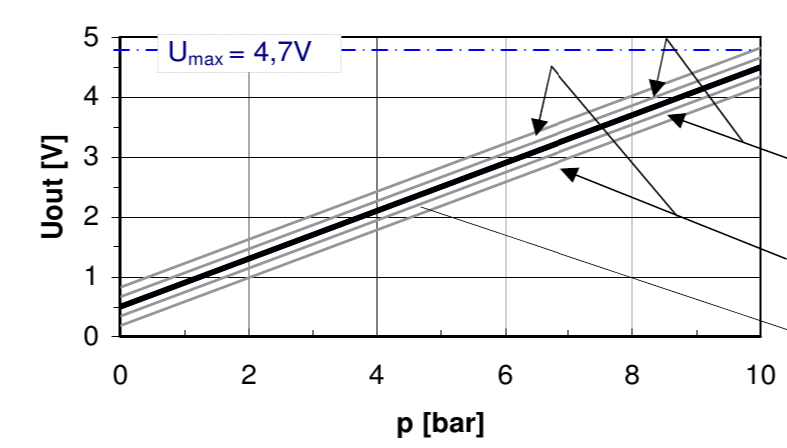
\includegraphics[width=\textwidth]{assets/specs/adc_product_specs.png}
            \caption{\it Product Specifications for CWS}
        \end{figure}
        \vspace{0.2cm}
    \end{minipage}
\end{frame}

%==============================================================================
% DESIGN AND IMPLEMENTATION SECTION: Embedded Linux
%==============================================================================

\subsection{Embedded Linux With Yocto Project}
% Consolidation slide since we need to go faster
\begin{frame}
  \frametitle{Embedded Linux and The Yocto Project}
  \begin{columns}
    \column{0.475\textwidth}
    \begin{block}{Embedded Linux}
      \begin{itemize}
        \item Industry standard for embedded Operating system
        \item Rich ecosystem of open-source tools and software
      \end{itemize}
    \end{block}
    \column{0.475\textwidth}
    \begin{block}{The Yocto Project}
      \begin{itemize}
        \item Collection of tools to build a custom embedded Linux distribution
        \item Fine-grain control of every aspect of deployed image
      \end{itemize}
    \end{block}
  \end{columns}
\end{frame}

\begin{frame}
  \frametitle{Embedded Linux}
  \begin{figure}
    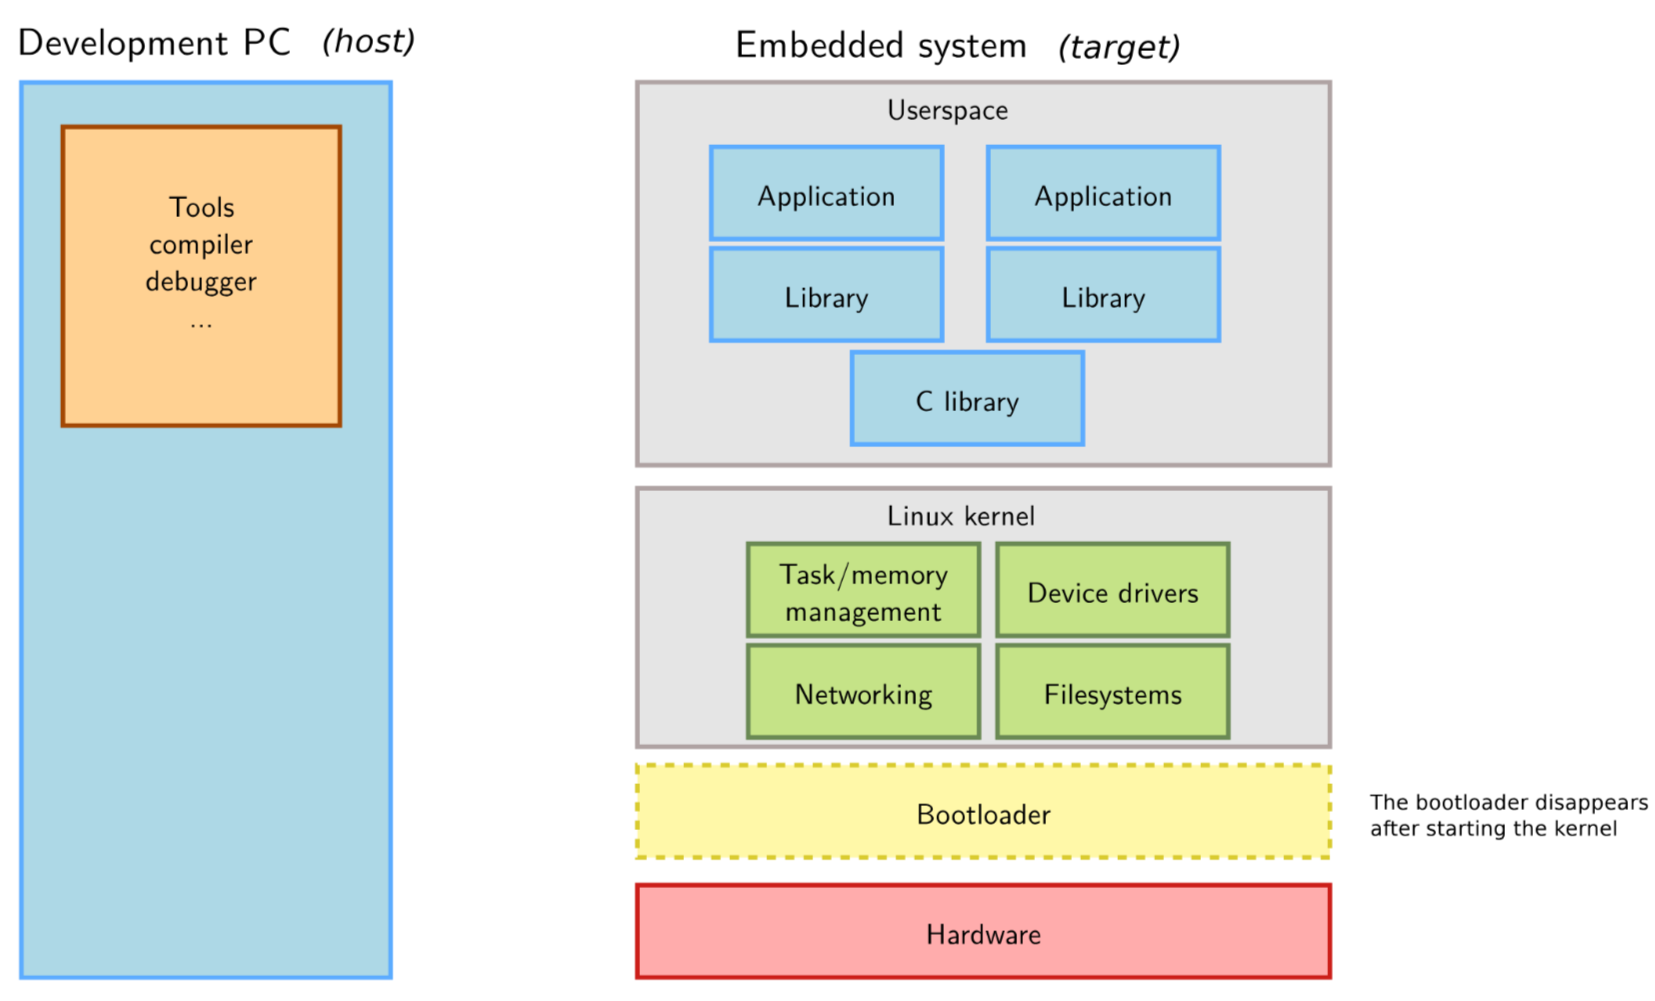
\includegraphics[width=175px]{assets/diagrams/embedded_linux.png}
    \centering
    \caption{\tiny Source:\underline{\href{https://bootlin.com/}{https://bootlin.com/}}\hspace{\textwidth}
    \textit{Embedded Linux system architecture}}
  \end{figure}
  \vspace{-16px}
  \begin{block}{Why use embedded Linux?}
    \small{
      \begin{itemize}
        \item Industry standard for any embedded operating system
        \item Access to open-source software (OSS) and tools
        \item Networking and connectivity made easy 
        \item Easily save/access data with filesystem
      \end{itemize}
    }
  \end{block}
\end{frame}

\begin{frame}
  \frametitle{Using The Yocto Project to Build a Custom Distribution}
  \begin{minipage}{0.475\textwidth}
    \begin{block}{What is the Yocto Project and why?}
        \begin{itemize}
          \item Most popular set of tools for embedded Linux Development
          \item Collection of OSS tools to make a custom Linux distribution
          \item Independent of target architecture
          \item \DarkBoldP{bitbake} build tool handles \LightBold{metadata}
          \item \LightBold{MetaData} can be in the form of 
            \begin{itemize}
              \item software build/patch instructions
              \item configuration files for software
            \end{itemize}
          \item \LightBold{MetaData} organized in its \LightBold{Layer Model}
        \end{itemize}
    \end{block}
  \end{minipage}
  \hfill
  \begin{minipage}{0.475\textwidth}
    \begin{figure}
      \center
      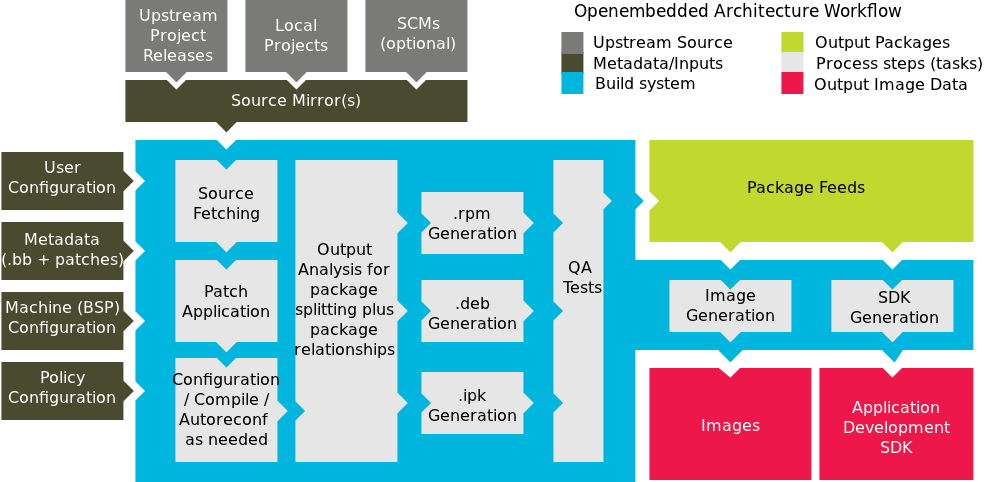
\includegraphics[width=180px]{assets/diagrams/yocto-environment.png}
      \caption{Source: \href{https://docs.yoctoproject.org}{https://docs.yoctoproject.org}\hspace{\textwidth}
      \it High-level diagram representing how builds work using The Yocto Project}
    \end{figure}
  \end{minipage}
\end{frame}

\begin{frame}
  \frametitle{Custom Linux Image for the STM32MP1-DK2}
  \begin{minipage}{0.475\textwidth}
    \begin{block}{What is used in the deployed image?}
      \begin{itemize}
        \item ST's BSP (board support package) layer provides metadata 
          \begin{itemize}
            \small
            \item Hardware drivers
            \item Kernel Configurations
            \item Devicetree
          \end{itemize}
        \item Custom layer \DarkBoldP{meta-zf-project}
          \begin{itemize}
            \small
            \item \DarkBold{nginx} (webserver), \DarkBold{wpa\_supplicant} (Wi-Fi access client/
              IEEE 802.1X supplicant)
            \item recipes for custom applications (Web application, Server, Cortex-M4 Firmware)
            \item Kernel configurations and custom Devicetree
          \end{itemize}
      \end{itemize}
    \end{block}
  \end{minipage}
  \hfill
  \begin{minipage}{0.5\textwidth}
    \begin{figure}
      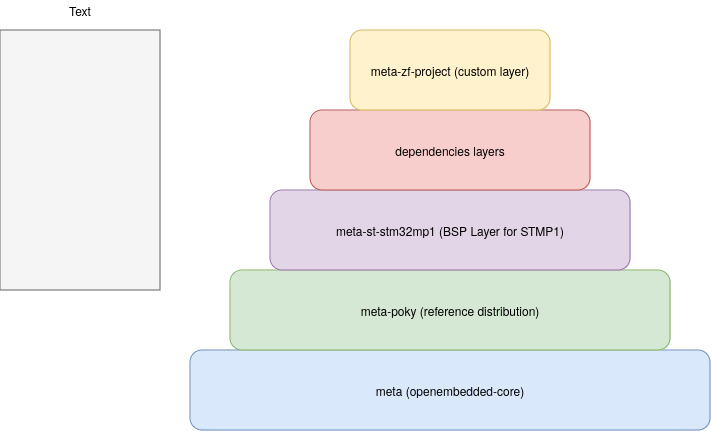
\includegraphics[width=1.125\textwidth]{assets/diagrams/layers.png}
      \caption{\it Layer Model representation of this project for deploying onto a 
      STM32MP1-DK2}
    \end{figure}
  \end{minipage}
\end{frame}

%==============================================================================
% DESIGN AND IMPLEMENTATION SECTION: IPC with OpenAMP
%==============================================================================
\subsection{Inter-Processor Communication}
\begin{frame}
  \frametitle{Inter-Process Communication on a Heterogenous Architecture}
  With a heterogenous architecture (ARM Cortex-A7 and ARM Cortex-M4) how can information be shared?\\
  {\em \scriptsize Hetergenous multiprocessor SoCs cannot directly communicate }
  \break
  \begin{minipage}{0.465\textwidth}
    \begin{block}{OpenAMP (Asymmetric Multi-Processing) Project}
      \footnotesize
      \begin{itemize}
        \item Software framework that places standard protocol for shared memory
        \item Implemented on top of \DarkBoldP{virtio} framework
        \item STM provides \DarkBoldP{virt\_uart} driver for recieving/transmitting messages
          over \DarkBoldP{RPMsg protocol}
        \item STMP1 layer automatically enables the \DarkBoldP{RPMSG tty driver} kernel module
          \begin{itemize}
              \tiny
            \item creates file in Linux filesystem: \DarkBoldP{/dev/ttyRPMSG<X>}
            \item can read and write to like a normal file
          \end{itemize}
        \item \DarkBoldP{remoteproc} framework allows dynamic and remote loading of Cortex-M4 firmware
        \item \LightBold{Resource Table} defined in firmware opens a trace in\\
          {\scriptsize\DarkBoldP{/sys/kernel/debug/remoteproc/remoteproc0/trace0}}
          \begin{itemize}
              \tiny
            \item Used for logging measured data in CSV format
          \end{itemize}
      \end{itemize}
    \end{block}
  \end{minipage}
  \hfill
  \begin{minipage}{0.465\textwidth}
    \begin{figure}
      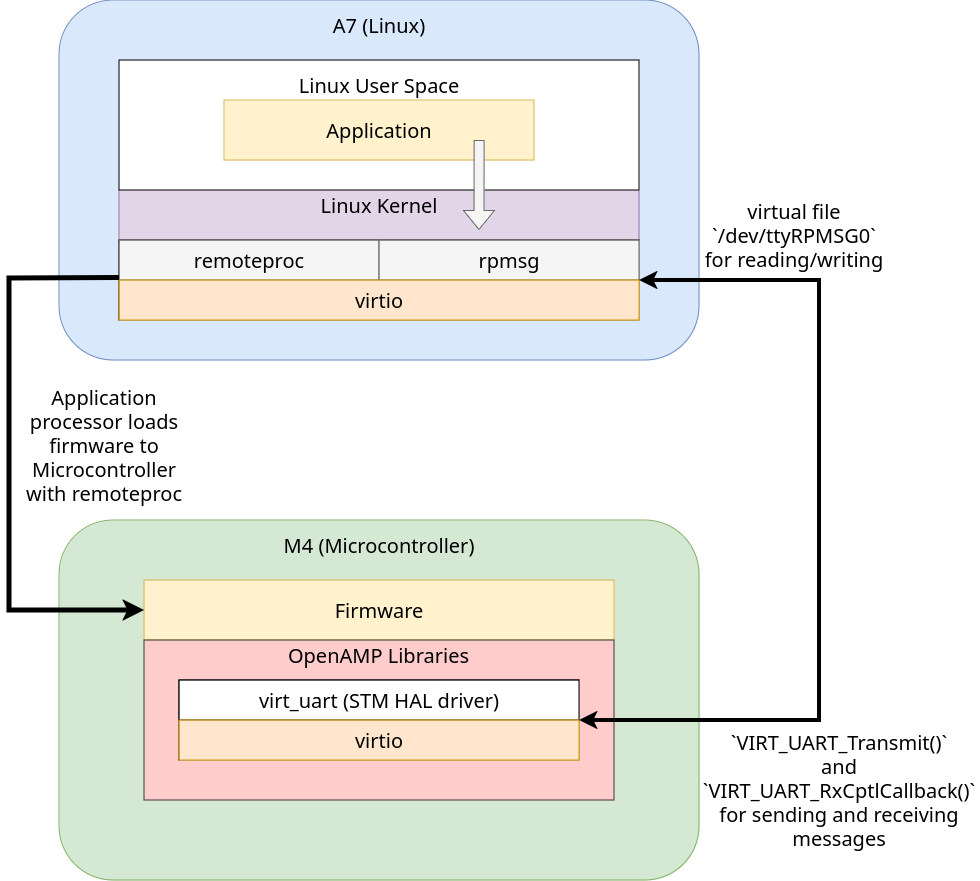
\includegraphics[width=\textwidth]{assets/diagrams/ipc.drawio.png}
      \caption{Inter-processor communication between Cortex-A7 (Linux) and Cortex-M4 (Microcontroller)}
    \end{figure}
  \end{minipage}
\end{frame}

%==============================================================================
% DESIGN AND IMPLEMENTATION SECTION: Rust
%==============================================================================
\subsection{Web Application and Server}
\begin{frame}
  \frametitle{Rust}
  \begin{minipage}{0.75\textwidth}
    The Rust programming language was used to write both major \\ 
    applications (web-based application and web server) for 2 main \\ reasons.
  \end{minipage}
  \hfill
  \begin{minipage}{0.20\textwidth}
    \begin{figure}
      
\includegraphics[width=\textwidth]{assets/misc/rewrite-it-in-rust.jpg}
      \caption{\it Ferris, universally accepted mascot of the Rust Programming language}
    \end{figure}

  \end{minipage}
  \hfill
  \vspace{-8px}
  \begin{block}{Memory Safety and Performance}
    \begin{itemize}
      \item A set of rules called \DarkBold{Ownership} enforced by compiler to prevent memory leaks
      \item \DarkBold{Borrow checker} within the compiler prevents programs unsafe programs from compiling*
      \item Nearly as or just as performant as C with \DarkBold{Zero Cost Abstractions}
      \item Advocated by/used by several United States goverment agencies:
        \begin{itemize}
          \item \LightBold{National Security Agency (NSA)} and 
            \LightBold{Cybersecurity and Infrastructure Security Agency (CISA)}
          \item \LightBold{Defense Advance Research Projects Agency} 
          \item \LightBold{The White House}
        \end{itemize}
    \end{itemize}
  \end{block}
\end{frame}

%==============================================================================
% DESIGN AND IMPLEMENTATION SECTION: Web-Assembly Application and Server
%==============================================================================

\begin{frame}
  \frametitle{Web-Application for User Interface}
  \begin{minipage}{0.5\textwidth}
    \begin{block}{Web Application in WebAssembly (WASM)}
      \begin{itemize}
        \item WASM is a compiled, binary format executable 
        \item Much faster than traditional Javascript programs
        \item Using the Yew framework, written in Rust
      \end{itemize}
    \end{block}
    \begin{block}{Web application Features}
      \begin{itemize}
        \item Shows if application is connected to associated server
        \item Selection of different devices
        \item Shows progress and state of test
        \item Allows download to results in a CSV
      \end{itemize}
    \end{block}
  \end{minipage}
  \hfill
  \begin{minipage}{0.4\textwidth}
    \begin{figure}
      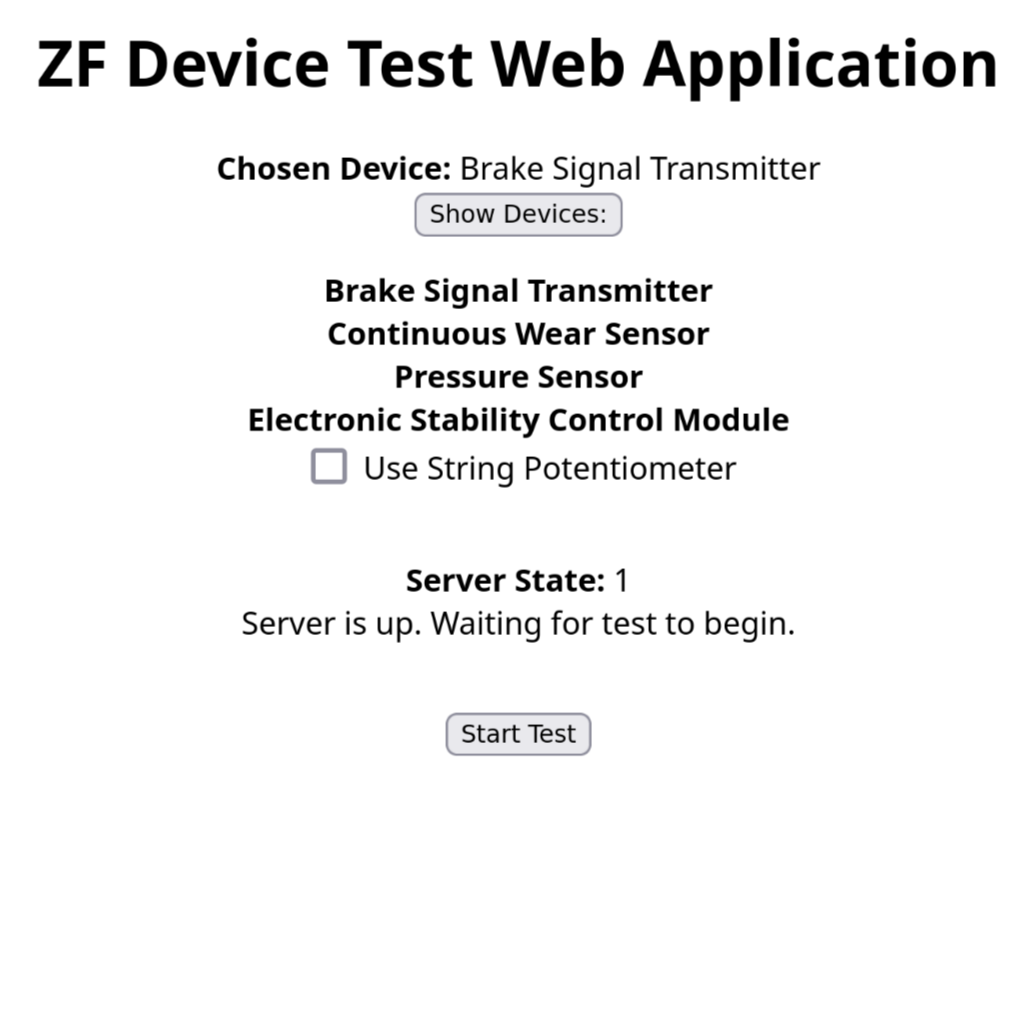
\includegraphics[width=\textwidth]{assets/misc/webapp.png}
      \caption{\it Web application with dropdown selection of different devices}
    \end{figure}
  \end{minipage}
\end{frame}

\begin{frame}
  \frametitle{Custom API Web Server}
  \begin{minipage}{0.5\textwidth}
    \begin{block}{Web Server features}
      \begin{itemize}
        \item Handles \DarkBoldP{HTTP requests} from web application
        \item Dynamically loads M4 Firmware for selected device with \DarkBoldP{remoteproc}
        \item Polls for results by reading and writing to \DarkBoldP{/dev/ttyRPMSG0} 
        \item Saves information from \DarkBoldP{/sys/kernel/debug/remoteproc/remoteproc0/trace0} as CSV for download
      \end{itemize}
    \end{block}
  \end{minipage}
  \hfill
  \begin{minipage}{0.4\textwidth}
    \begin{figure}
      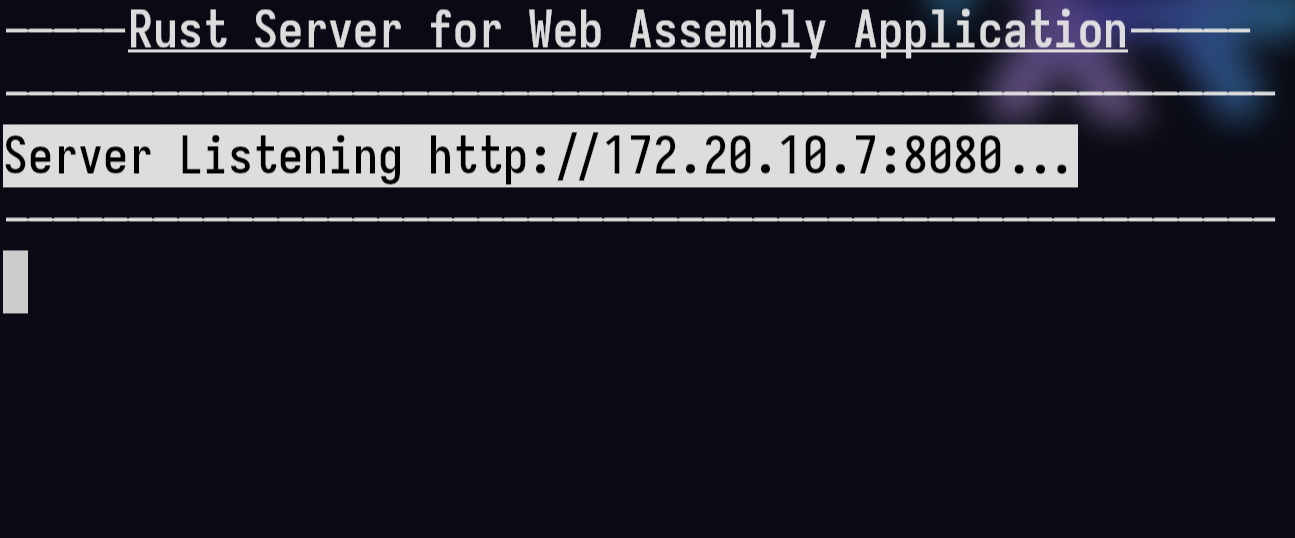
\includegraphics[width=\textwidth]{assets/misc/server1.png}
      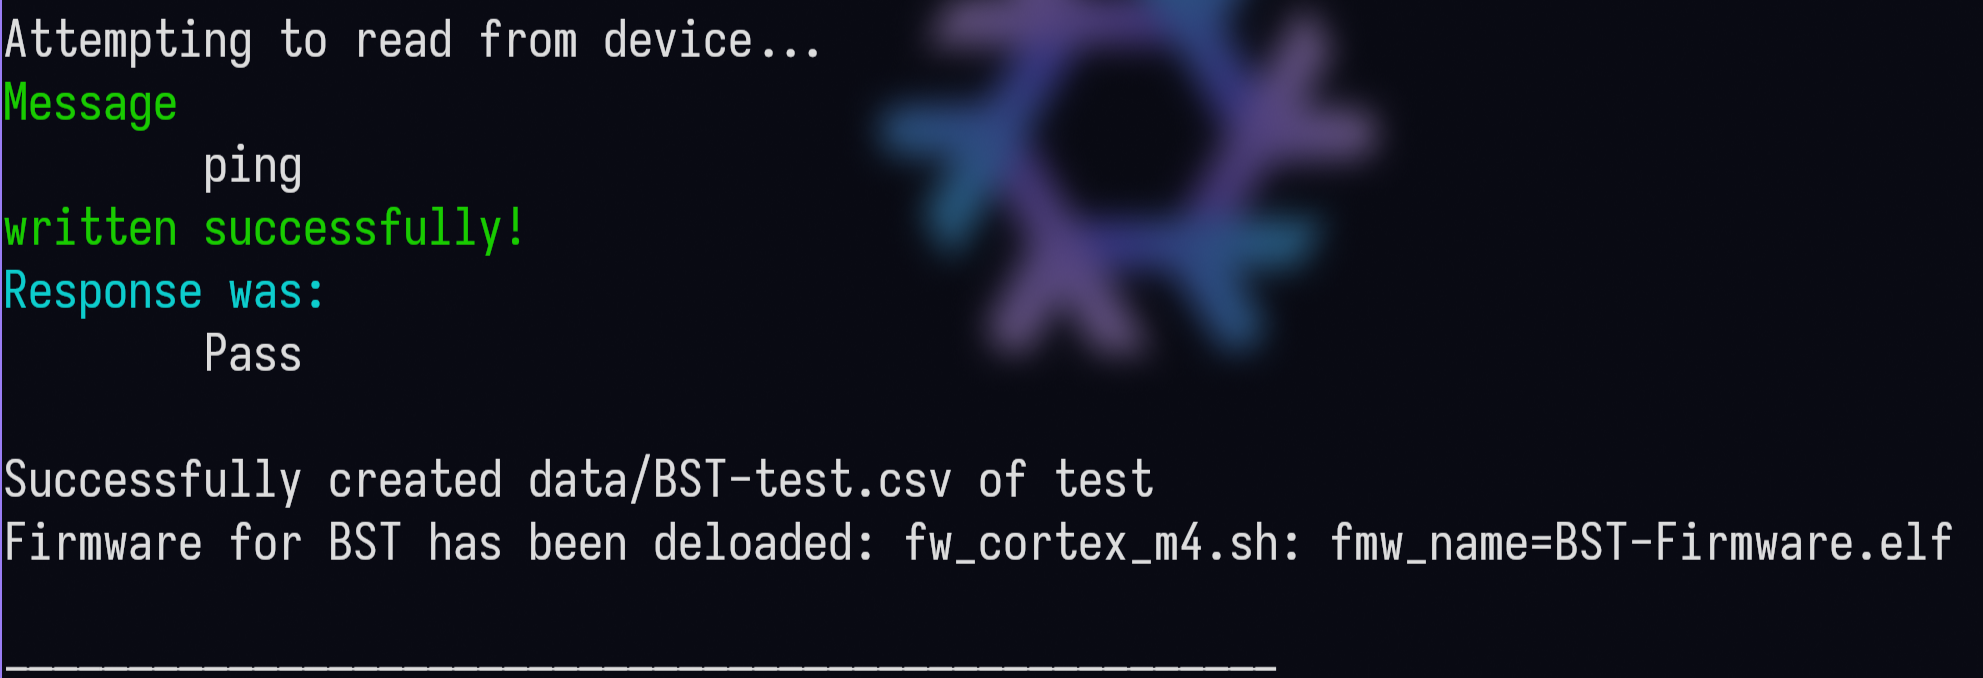
\includegraphics[width=\textwidth]{assets/misc/server2.png}
      \caption{\it Console logging of server application}
    \end{figure}
  \end{minipage}
\end{frame}

\begin{frame}
  \frametitle{Software Architecture}
  \begin{figure}
    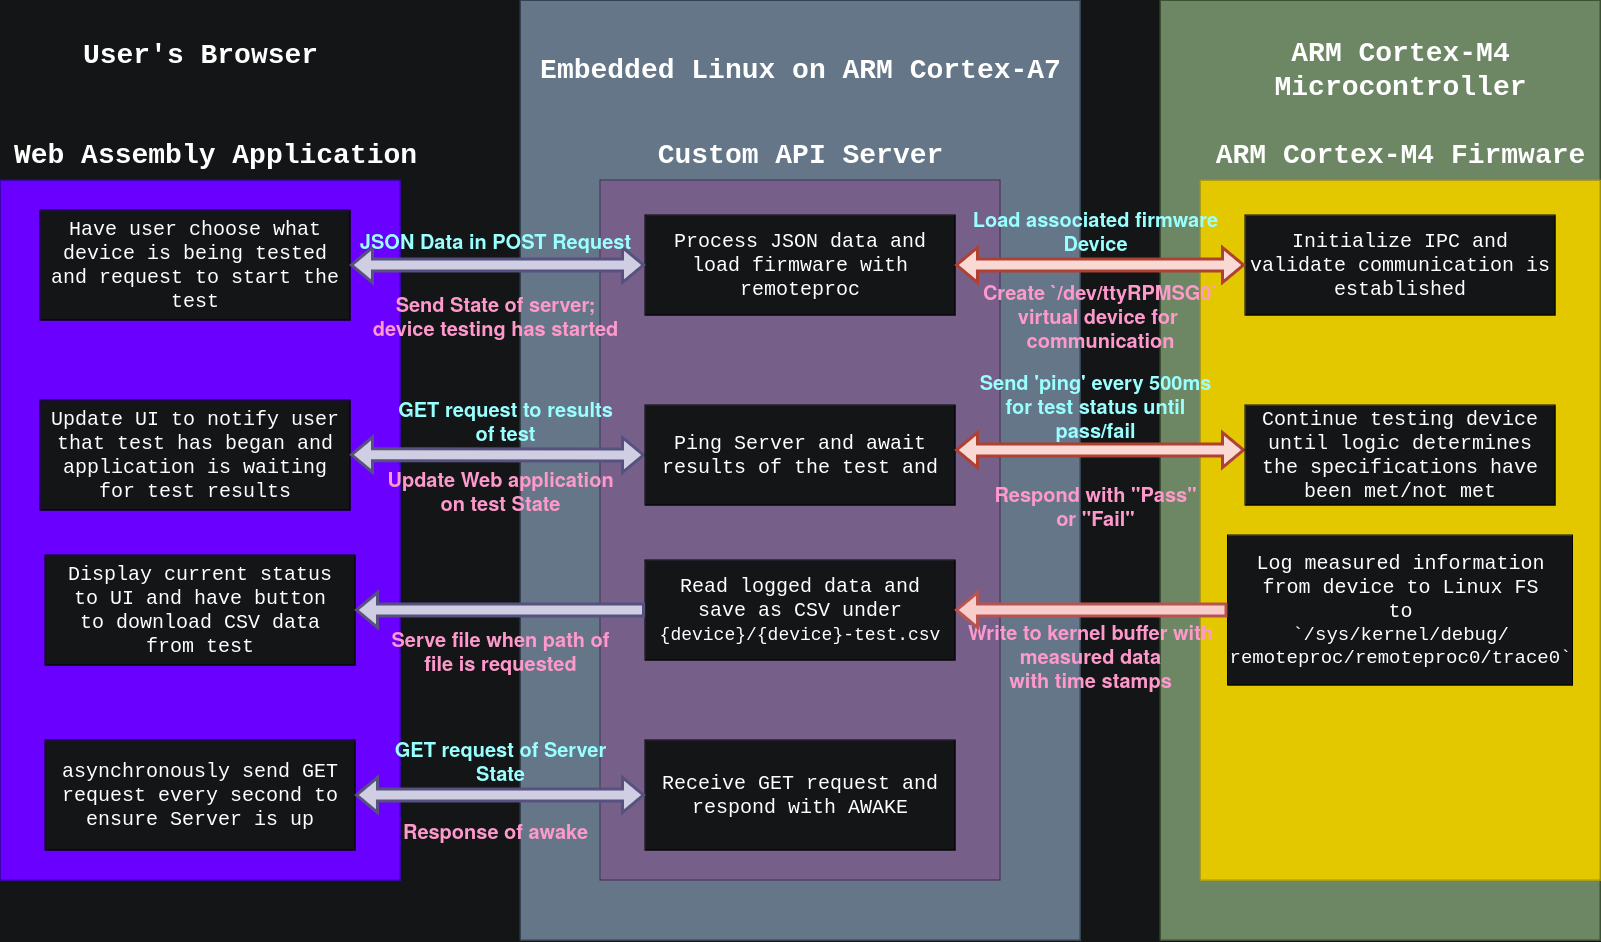
\includegraphics[height=0.825\paperheight]{assets/diagrams/software_stack.drawio.png}
  \end{figure}
\end{frame}

\section{Verification}
\begin{frame}
  \begin{block}{Link to video demonstration}
    \href{https://dylxndy.xyz/senior-design-presentation/verification}
    {\color{lime}{\ul{https://dylxndy.xyz/senior-design-presentation/verification}}}
  \end{block}
\end{frame}

\section{Challenges}
\begin{frame}
  \frametitle{Challenges}
  \begin{itemize}
    \item System Clock configuration with Devicetree
    \item Timer configuration for PWM signals
    \item Mini-360 Buck Converter
    \item PCB Creation
  \end{itemize}
\end{frame}

\section{Future Work}
\begin{frame}
  \frametitle{Future Work}
  \begin{itemize}
    \item Finish CAN implementation for ESCM
      \begin{itemize}
        \item USB to CAN used currently
        \item enabled \DarkBoldP{CAN\_GS\_USB} module in Linux Kernel
      \end{itemize}
    \item Improve Web application appearance
  \end{itemize}

\end{frame}

\section{Closing}
\begin{frame}
  \frametitle{Special Thanks}
  \begin{itemize}
    \item Dr. Grantner (faculty advisor)
    \item David Florida (lab technician)
    \item Patrick McNally (Head of Engineering at ZF Group - Auburn Hills, MI)
    \item Davis Roman (Senior Staff Software Engineer at Rivian - Palo Alto, CA)
  \end{itemize}
\end{frame}

\begin{frame}
  \frametitle{Thank you}
  Any Questions?
  \begin{block}{Project Sources}
    \begin{itemize}
      \item \DarkBoldP{Custom Yocto Project Layer:}
        \begin{itemize}
          \item \url{https://github.com/DMGDy/meta-zf-project}
        \end{itemize}
      \item \DarkBoldP{Custom Web Server in Rust} 
        \begin{itemize}
          \item \url{https://github.com/DMGDy/zf-webserver-app}
        \end{itemize}
      \item \DarkBoldP{Web Application in WASM}
        \begin{itemize}
          \item  \url{https://github.com/DMGDy/zf-yew-app}
        \end{itemize}
      \item \DarkBoldP{Microcontroller Firmware}
        \begin{itemize}
          \item \url{https://github.com/danb127/Brake-System-Tester}
        \end{itemize}
      \item \DarkBoldP{This Presentation}
        \begin{itemize}
          \item \url{https://github.com/DMGDy/ECE4820-Presentation}
        \end{itemize}
    \end{itemize}
  \end{block}
\end{frame}

\end{document}
